%\documentclass[a4j,12pt,twocolumn]{jsik}
\documentclass[12pt,a4paper,twocolumn,twoside]{jsik}
%\usepackage{url}

\usepackage{cite}
\usepackage{amsmath,amssymb,amsfonts}
\usepackage{algorithmic}
\usepackage{graphicx}
\usepackage{textcomp}
\usepackage{xcolor}

\usepackage{float}

\begin{document}

\pagestyle{empty}
\thispagestyle{empty}

\articletype{研究論文}
%日本語タイトル
\jtitle{基底選択を用いた話題性の評価}
%英語タイトル
\etitle{Topic Estimation Method Using Base Selection}

\jauthor{輪島 幸治$^{\dag}$ 古川 利博$^{\dag\dag}$ 佐藤 哲司$^{\ddag}$}
\eauthor{Koji WAJIMA Toshihiro FURUKAWA Tetsuji SATOH}
\affiliation{
$^{\dag}$ 筑波大学 図書館情報メディア研究科 \\
Graduate School of Library, Information and Media Studies, University of Tsukuba \\
〒305-8550 茨城県つくば市春日1-2 \\
E-mail: kwajima@ce.slis.tsukuba.ac.jp \\
$^{\dag\dag}$ 東京理科大学 工学部情報工学科 \\
〒125-5846 東京都葛飾区新宿6-3-1\\
Dept.Information and Computer Technology., Science University of Tokyo
%EMail: email-addr@example.jp \\
\\
$^{\ddag}$ 筑波大学 図書館情報メディア系 \\
Faculty of Library, Information and Media Science, University of Tsukuba \\
〒305-8550 茨城県つくば市春日1-2 \\
E-mail: satoh@ce.slis.tsukuba.ac.jp \\
}

\jabstract{
%(400文字以内)
%511文字
%--------------------
%現状分析
近年,ユーザが情報発信する
CGM(Consumer Generated Media) や
ソーシャルメディアが台頭する情報化社会へと移行してきている.
%
%課題提示
商品やサービスの利用者であるユーザが情報交換を行う
オンラインコミュニティは誰もが質問・回答できる利点がある.
オンラインコミュニティは,誰もが閲覧できる環境であることから
投稿された質問記事に対して,適切な対応をとり続けることが,
炎上などの社会的な影響を回避する上で不可欠となっている.
%
%解決策の提示
本論文では,オンラインコミュニティに投稿された質問記事から,
記事が言及している話題性を評価するのに
有効な基底の選択手法を提案する.
%
%提案法の特徴
提案手法は,非負値行列因子分解(NMF)による特徴量変換および基底選択で構成されている.
提案手法では,既存研究のテキスト情報の特徴量である
表層情報,語種や品詞,文末表現など2,000次元を越える特徴量を用いる.
%
%分かったこと
提案手法はを複数のオンラインコミュニティ記事に適用し,
サポートベクタ回帰モデル(SVR)と分類器を用いて評価した結果,
基底選択の有効性が確認できたので報告する.
%--------------------
}

\eabstract{
%ここ数年の間,コンシューマとメーカ間のコミュニケーションについて,社会的関心が高まってきている.
The social concern with communication between a consumer and maker has been growing for the last several years.
%
%インターネットでは,オンラインメディアのコミュニケーションは不特定多数のユーザによって調査されている.
A large number of unspecified users are investigating Consumer Generated Media's communication on the Internet.
%
%Consumer Generated Mediaにおけるクレームが購買行動に影響を与える影響は大きい.
The claim has the tremendous impact on the purchasing behavior in Consumer Generated Media.
%
%この論文の狙いは,話題性予測に影響が大きい特徴量の調査研究にある.
This paper is intended as an investigation of significant feature quantity for topic forecast.
%
%本論文はオンラインコミュニティの投稿記事で話題性を調査する.
In this Paper, We investigate online media's topic forecast on Online Community article.
%
%我々は既存研究を用いてテキスト情報の特徴量を網羅的に抽出した.
We comprehensively extracted text information's feature quantity using existing research.
%
%テキスト情報の特徴量には31個,2,071次元を用いる.
Feature quantity is used, for 31 types and 2,071 dimensions in text information.
%
%提案手法は,NMFによる特徴量変換および基底の評価で構成されている.
Proposed Method consists of feature transformation and the base on evaluation using Nonnegative Matrix Factorization (NMF).
%
%提案手法の有効性はSVRと分類器で評価する.
The validity of the Proposed Method is verified by Support Vector Regression (SVR) and Classifiers.
%
%評価結果から,閲覧数に影響を与える特徴量がわかった.
It was found from the evaluative result that have an impact on view count.
%
%研究結果を報告する.
We report that research result.
}

\keywords{
NMF,LSI,LDA,SVR,質問記事
}

\maketitle

%1
\section{はじめに}
%現状分析
近年,CGM(Consumer Generated Media)や
ソーシャルメディアが台頭する情報化社会へと移行してきている.
%
例えば,ソーシャルメディアの情報は,
企業の評判分析など多様な分野で用いられている
\footnote{Oracle Help Center - Cloud Documentation : \\
https://docs.oracle.com/en/cloud/saas/index.html}.\\
%
%課題提示
CGMやソーシャルメディアなどのオンラインコミュニティは
誰もが気軽に閲覧・質問・回答が行える.\\
このため,情報収集や気楽なコミュニケーション,
時間をかけた議論など目的に応じた様々な利点が示されている.
%
また,商品やサービスの利用者が,
内容や使い勝手などの情報交換も盛んに行われている.
%
そこで共有・共感された価値ある情報は,
情報伝播や購買行動に影響を与えることが大きい.
%
共感に基づいた生活者消費行動モデルは,
SIPS(Sympathize Identify Participate Share \& Spread)
\cite{SIPS}
\footnote{
SIPSでは,生活者消費行動を
S(Sympathize : 共感する),
I(Identify : 確認する),
P(Participate : 参加する),
S(Share \& Spread : 共有・拡散する)とモデル化している.
SIPSモデルでは,共感に次ぐ重要な要素は,参加してもらうことである.
参加はエバンジェリスト(伝道者),ロイヤルカスタマー(支援者),ファン(応援者),
パーティシパント(参加者)など,
企業やブランドの生涯顧客価値を高めていく過程と重なっている.
}
\footnote{
SIPS : http://www.dentsu.co.jp/sips/index.html
}
と呼ばれる.
%
一方で,クレームや批判的なコメントも急激に広がる.
%
このため,企業は話題性やクレームがある
質問記事を検知・予測し,早急に対処することが欠かせない.

%解決策の提示
本研究では,質問記事における話題性の多寡を推定することを目的に
基底選択を用いた質問記事の評価手法を提案する.
%
本研究における質問記事の話題性は閲覧数が多い質問記事とする.
閲覧数が多いことは,多くの利用者が,
共感・関心を持って質問記事を閲覧している状態だと言える.
このため,質問記事の閲覧数に基づいて評価する.
%
異常や変化の兆しに基づく閲覧数に基づいた特徴が明らかになることで,コンテンツの内容で,
投稿後に話題になる質問記事を検知・予測することが期待できる.

%提案法の特徴
提案手法では,質問記事からできる限り多くの特徴量を抽出し,
非負値行列因子分解(NMF)によって,特徴量を変換する.
%
特徴量の変換後に得られる基底を
質問記事集合の特性に基づいて評価し,基底選択する.
%
本研究では,各質問記事で,コンテンツが異なる特性に着目した.
質問記事を高次元なベクトル化した場合,
0の多いスパースなベクトルになる傾向にある.
したがって,各コンテンツで,観測ベクトルは大きく異なる.
%
そこで,提案手法では,変換特徴量である基底に対する
各質問記事の重みに基づいて,
閲覧数が多いコンテンツにおける基底を評価した.
%
提案手法では,
既存研究におけるテキスト情報の特徴量を網羅的に抽出した
31個,2,071次元の特徴量を用いている.

\newpage
%評価結果
提案手法の有効性は
サポートベクタ回帰モデル(SVR)と分類器を用いて評価する.
SVRを用いた閲覧数の予測では
平均絶対誤差(MAE)および平均二乗平方根誤差(RMSE)の
評価指標で有効な結果が得られた.
また,分類器を用いた評価では,
適合率,再現率,F値の評価指標で有効な結果が得られた.

%論文の構成
本論文では2章で関連研究に関して述べる.
3章で提案手法である基底選択の評価手法を詳述する.
4章では,提案手法の実装と評価対象について述べ,
5章で実験結果を示す.
6章では,得られた結果に対する考察を論じる.
最後に7章でまとめと今後の課題を示す.

%2
\section{関連研究}
本研究では,オンラインコミュニティのコンテンツである
質問記事のテキスト情報から話題性の評価を試みた.
\ref{COMMUNITY}節および\ref{TOPIC_TREND}節で,
オンラインコミュニティおよび話題性に関する既存研究を概観する.
%
\ref{FEATURE}節,\ref{TOPIC}節,\ref{DIC}節で,
本研究で評価要素として用いる特徴量に関する研究を述べる.

%2.1
\subsection{cQAサイトを対象とした研究}\label{COMMUNITY}
本研究の対象は,情報発信メディアの一つで,
ユーザが相互に質問・回答を行うオンラインコミュニティの
cQAサイト(Community based question-answering service)である.
%
cQAサイトを対象にした研究には,類似質問の同定,
回答の評価,要約の作成など数多くの研究がある\cite{article_okumura}.
%
質問記事内から特徴量を抽出し,
ベストアンサーを推定する研究\cite{article_yokoyama},
質問記事の文体に着目し,最適な回答を提示する研究\cite{article_kure},
質問記事に教師付き機械学習アルゴリズムを適用させ,
既存のナレッジベースから類似の質問記事を検索する研究\cite{article_han}などがある.
%
テキスト情報を用いたオンラインコミュニティの場合,
各オンラインコミュニティで投稿者が異なる.
したがって,投稿内容や特徴的な単語などは異なる.
本研究では,オンラインコミュニティの話題性が評価対象である.

%2.2
\subsection{話題性}\label{TOPIC_TREND}
オンライン上のメディアを対象とした
話題や動向の評価は,多くの評価方法がある.
既存研究では,質問記事のコンテンツであるテキスト情報から,
出現頻度や推移に着目した評価が行われることが多い.
評価では統計量や重要語などの要素が用いられる
\cite{trend,weblogs}.
%\cite{trend}\cite{weblogs}
%
また,ソーシャルブックマーク\footnote{
ソーシャルブックマークとは,編集したブックマークをインターネット上に公開できるウェブサイトである.
}を用いたブックマークの周期性の分析や検索の時期や検索結果のランキング手法の研究
\cite{discovering_periodicity_socialbookmark,reranking_method_socialbookmark},
ユーザーの潜在変数などのメタ情報を用いて情報伝播を分析する方法などがある\cite{information_diffusion_model}.
%\cite{discovering_periodicity_socialbookmark}\cite{reranking_method_socialbookmark},
%
加えて,話題性の流行や人気に影響を与える要素には,
コンテンツに加え,
クチコミ
\cite{buzz_mrk}
\footnote{インターネットでは,各種商品やサービスなどに関する利用者(消費者側) の評価・体験談の投稿など.}
や
共感
\cite{SIPS}
\footnote{他人の体験する感情を自分の体験のように感じること.}
,
技術のハイプ・サイクル(Gartner Hype Cycle)
\cite{gartner}
\footnote{新しいテクノロジが時間の経過と共にどのように発展していくのかのトレンドを示す先進テクノロジの成熟度と採用率のグラフ.}
\footnote{Gartner - Research \& Advisory Overview : 
\\https://www.gartner.com/en/research/methodologies}
などもある.
%
本研究では,オンラインコミュニティである
cQAサイト上の質問記事のテキスト情報を用いて,
特徴量を抽出・特徴量変換し,話題性の評価に適用する.

テキスト情報を用いた話題性評価の研究には,
トレンドキーワード(流行語)やトピックを用いた手法がある.
%
トレンドキーワードとは,検索エンジンやソーシャルメディアで,
利用者から興味関心が高いキーワードである.
検索エンジンの検索語であるクエリの頻度などで抽出が行われる.
%
トレンドキーワードのウェブリソース間の振る舞いに関する研究や,
コミュニティにおける発言割合の研究などがある\cite{trend_query_analysis,gradual_buzzwords}.
%\cite{trend_query_analysis}\cite{gradual_buzzwords}
%
\ref{TOPIC}節で後述するテキスト情報が言及する話題(トピック)を用いた手法では,
アルゴリズムでテキスト情報からトピックと呼ばれる単語集合を抽出し,
時系列や種別に基づいて流行や人気を評価する
\cite{topic_book,topic_burst}.
%\cite{topic_book}\cite{topic_burst}.
%
話題性の評価基準には,
トピックのバースト
\footnote{
特定の話題が起因して,トピックの頻度が急上昇することで検出される現象.}
度合い\cite{topic_burst}や
盛り上がりの早さや平均返信数\cite{article_matsumura},
ユーザ行動やコミュニティの成長率\cite{article_toriumi}などが用いられている.

%2.2
\subsection{テキスト情報の特徴量に関する研究}\label{FEATURE}
本研究で使用する既存研究のテキスト情報の特徴を表1に示す.
%
表1の特徴はいずれも文章の表層的な特徴であることから,
これらの特徴を表層情報と称する.
%
本研究の文字種は,ひらがな,カタカナ,漢字,アルファベット,
数字,半角記号,空白記号,全角記号の8個である.

\renewcommand\thefootnote{\fnsymbol{footnote}}
%
\begin{table}[htb]
  \caption{表層情報}
  \label{tab:dics_tag}
  \begin{center}
  \begin{tabular}{|c|c|c|l|} \hline
    {\bf 項番} & {\bf 特徴名} & {\bf 次元数} & \multicolumn{1}{|c|}{\bf 値の定義/例} \\ \hline\hline
   1 & 文数 & 1 & [。][?][!] \\
     &  &  & の合計頻度 \\ \hline
   2 & 読点 & 1 &  [、]の頻度 \\ \hline
   3 & 句点 & 1 & [。]の頻度 \\ \hline
   4 & 文長 & 1 & 文字数 \\ \hline
   5 & 文字種(1) & 8 & 各文字種の頻度\footnotemark[1] \\ \hline
   6 & 文字種(2) & 8 & 各文字種の比率\footnotemark[1] \\ \hline
   7 & 読点間距離 & 1 & 読点間の距離\cite{punctuation_mark} \\ \hline
   8 & 漢字含有率 & 1 & 漢字の包含率\cite{punctuation_mark} \\ \hline
  \end{tabular}
  \end{center}
\end{table}
%
\footnotetext[1]{Unicode 10.0 Character Code Charts \\http://www.unicode.org/charts/}
%
\renewcommand\thefootnote{\arabicl{footnote}}

%2.3
\subsection{話題抽出に関する研究}\label{TOPIC}
テキスト情報の特徴量に関する研究に,話題抽出がある.
話題抽出で用いられる基本的なアルゴリズムには,
潜在意味解析(LSI : Latent Semantic Indexing)と
トピックモデル(LDA : Latent Dirichlet Allocation)がある\cite{topic_book}.
%
潜在意味解析やトピックモデルを適用し,
得られる結果は類似した語彙の集合であり,
本研究で述べる話題に相当する.
以下,特に断らない場合は,
本研究では話題抽出アルゴリズムの結果をトピックとし,
話題あるいは話題抽出を言う.
%
潜在意味解析やトピックモデルの詳細は,
文献\cite{topic_book}にゆずり,
ここでは,概略を述べるに留めることにする.

話題抽出のアルゴリズムを適用する文書集合は,
1行が1文書,各列は語彙に相当し,
要素は語彙Vの出現頻度を持つ行列Nである.
%
LSIは,文書集合を低ランク行列の積
U$^{\mathrm{T}}$Hにそれぞれの行列の要素を二乗し,
総和をとったものが最小になるように行列分解する手法である.
%
$U = (u_{1}, \cdots , u_{D})$は,K行D列の重み付き係数行列である.
$H = (h_{1}, \cdots , h_{V})$は,K行V列の語彙行列である.
重み付き係数行列におけるUの要素は,文書に対する次元Kの重みに相当する.
本研究のLSIの特徴量は,Uの要素を用いた.

\newpage
LDAは,文書$w_{d}$が低ランク行列$\phi$と$\theta$をパラメータとして持つ
カテゴリ分布から生成されると仮定する手法である.
%
パラメータ$\theta_{d}$はトピック分布,パラメータ$\Phi$は単語分布集合である.
%
本研究のLDAの特徴量は,文書集合Nに対し,LDAを適用し得られるトピックK
の各文書の割り当て確率であるトピック分布$\theta$である.

LSIにおける低ランク行列の次元数K
およびLDAにおけるトピック数Kが話題に相当する.
%
LSIの次元数やLDAのトピック数は任意に設定できるが,
\ref{simulation}節で詳述するが,
本論文では十分に大きな値300とした.
%
話題の特徴量を表\ref{tab:topic_tag}に示す.
%
\begin{table}[htb]
  \caption{話題の特徴量の詳細}
  \label{tab:topic_tag}
  \begin{center}
  \begin{tabular}{|c|c|c|c|} \hline
    項番 & 特徴名 & 次元数 & 文献 \\ \hline \hline
    1 & LSI & & \\
     & (重み付き係数$u_{D}$) & 300 & \cite{topic_book,lsi_required} \\ \hline
    2 &LDA & & \\
     & (トピック分布$\theta_{d}$) & 300 & \cite{topic_book,lsi_required} \\ \hline
  \end{tabular}
  \end{center}
\end{table}

%2.4
\subsection{意味情報に関する研究}\label{DIC}
意味情報は,個々の研究で言語や形態論に基づき,
異なる特徴が用いられている\cite{reduplicated}.
%
本研究においては,
社会システム理論のゼマンティクという概念に基づき,
既存研究の辞書を用いる\cite{Luhmann}.
%
ゼマンティクとは,高度に一般化され,
状況に依存せずに使用できる意味である.
既存研究の辞書を用いることで,
状況に依存せずに意味情報が特徴量として抽出できる.
%
本研究では,学術目的の言語資源として,
従来研究で作成された日本語の辞書のうち,
言語資源の利用事例や応用研究がある既存辞書21個を選定した.
%
本研究で用いる21個の辞書を表\ref{tab:sentiment_tag}に示す.

%表\ref{tab:sentiment_tag}のうち,
%項番$15$の拡張固有表現の辞書は,
%関根の拡張固有表現階層の定義に基づき,
%Wikipedia の見出し語に対し,固有表現クラスを付与した辞書である.
表\ref{tab:sentiment_tag}の,
項番$15$の拡張固有表現の辞書は,
関根の拡張固有表現階層の定義に基づき,
Wikipedia の見出し語に対し,固有表現クラスを付与した辞書である.
%
また,項番$18$-$20$で用いている
単語感情極性対応表では,日本語の辞書の見出し語と読みを用いた.

加えて,表\ref{tab:sentiment_tag}の
項番$1$-$7$の辞書は調査研究目的に作成された辞書に基づいている.
%
項番$1$,$3$,$6$の辞書は意味分類体語彙表,
項番$2$,$5$の辞書は日本語教育基本語彙,
項番$4$,$7$の辞書は分類項目一覧表である.
\newpage

%
本研究では,下記に記載の基準で,辞書の加工および見出し語を選定した.
%
\begin{enumerate}
{\bf \item 見出し語の加工}
\\空白記号,「-」「0」「など」を除去

%\item 対象外の見出し語
{\bf \item 対象外の見出し語}
\\「」「-」「〔」「→」「/」「(」「・」「その他」\\を含む語
\end{enumerate}

\renewcommand\thefootnote{\fnsymbol{footnote}}
\begin{table}[htb]
  \caption{既存研究の特徴量の詳細}
  \label{tab:sentiment_tag}
  \begin{center}
  \begin{tabular}{|c|c|c|c|c|c|} \hline
    項番 & 特徴名 & 次元数 & 文献 \\ \hline \hline
    1 & 語種 & 7 &\footnotemark[2],\cite{moji_word_type_3} \\ \hline
    2 & 基本語(1) & 2 & \footnotemark[2],\cite{basic_vocabulary} \\ \hline
    3 & 基本語(2) & 6 & \footnotemark[2],\cite{basic_vocabulary} \\ \hline
    4 & 基本語(3) & 2 & \footnotemark[2],\cite{basic_vocabulary} \\ \hline
    5 & 意味分類(1)  & 233 &\footnotemark[2],\cite{semantic_attributes} \\ \hline
    6 & 意味分類(2)  & 487 &\footnotemark[2],\cite{semantic_attributes} \\ \hline
    7 & 意味分類(3)  & 307 &\footnotemark[2],\cite{semantic_attributes} \\ \hline
    8 & 機能表現  & 122 &\footnotemark[3],\cite{factuality_annotation} \\ \hline
    9 & 文末モダリティ  & 32 &\cite{modality} \\ \hline
    10 & 質問文末表現  & 38 &\cite{qa_feature} \\ \hline
    11 & IPA品詞  & 14 &\footnotemark[4],\cite{applied_proper_noun} \\ \hline
    12 & 固有名詞 & 4 &\footnotemark[4],\cite{applied_proper_noun} \\ \hline
    13 & 名詞比率  & 1 &\cite{applied_part_of_speech} \\ \hline
    14 & MVR  & 1 &\cite{applied_part_of_speech} \\ \hline
    15 & 拡張固有表現 & 132 &\footnotemark[5],\cite{extended_namedentity} \\ \hline
     & 評価極性情報 &  &\\ 
    16 & (用言編)  & 4 &\footnotemark[3],\cite{sentiment_verbs} \\ 
    17 & (名詞編)  & 51 &\footnotemark[3],\cite{sentiment_nouns} \\ \hline
     & 感情極性 &  & \cite{sentiment_spin} \\ 
    18 & (頻度)  & 2 & \footnotemark[6],\cite{sentiment_spin,sentiment_survey} \\ 
    19 & (比率)  & 2 & \footnotemark[6],\cite{sentiment_spin,sentiment_survey} \\ 
    20 & (平均値)  & 1 & \footnotemark[6],\cite{sentiment_spin,sentiment_survey} \\ \hline
    21 & 評価値表現 & 1 & \footnotemark[7],\cite{sentiment_fe} \\ \hline
  \end{tabular}
  \end{center}
\end{table}
%
%\cite{sentiment_spin}\cite{sentiment_survey}
\footnotetext[2]{『日本語教育のための基本語彙調査』データ \\http://mmsrv.ninjal.ac.jp/bvjsl84/}
\footnotetext[3]{機能表現タグ付与コーパス,日本語評価極性辞書 \\http://www.cl.ecei.tohoku.ac.jp/index.php}
\footnotetext[4]{ipadic version 2.7.0 ユーザーズマニュアル \\http://chasen.naist.jp/snapshot/ipadic/ipadic/doc/ipadic-ja.pdf}
\footnotetext[5]{NAIST Japanese ENE Dictionary on Wikipedia \\https://github.com/masayu-a/NAIST-JENE}
\footnotetext[6]{単語感情極性対応表 \\http://www.lr.pi.titech.ac.jp/\~takamura/pndic\_ja.html}
\footnotetext[7]{評価値表現辞書 \\http://www.syncha.org/evaluative\_expressions.html}
%
\renewcommand\thefootnote{\arabic{footnote}}

本研究における意味情報は,表\ref{tab:sentiment_tag}で示した
項番$1$の語種,項番$2$-$4$の基本語,
項番$5$-$7$意味属性,項番$8$の言語表現,
項番$9$の文末表現,項番$11$-$14$の品詞,項番$15$の固有表現,
項番$16$-$21$の評価表現の8個を評価に用いる.

%3
\section{提案手法}

%3.1
\subsection{概要}
オンラインコミュニティでは,
多くのユーザが閲覧するため,社会的な影響も大きい.
%
閲覧数が多い質問記事は,多くのユーザの疑問を解消,
あるいは興味と合致した重要な質問記事であると言える.
%
提案手法では,
重要な質問の判別に有効な基底選択の手法を提案する.

本研究ではグレゴリー・ベイトソン
\footnote{
アメリカの人類学者(1904-1980),民族誌「ナベン」「バリ」や人間関係論におけるダブル・バインド論など,
文化とパーソナリティ,コミュニケーションに関する理論で,学際的な功績を残した.
}
の情報の定義に着目している.
ベイトソンは情報を「``違い''を生む``違い''」
であると定義している\cite{definition_information}.
%
``違い''を土地と地図の差異に例えた場合,
土地には,高低,建造物,人口の分布など,
多様な要素がある\cite{what_information}.
また,土地が違えば地図も異なる.
地図には,高低図,街の配置図,人口分布図などがある.
%
地図は土地の特定の要素を選択した結果である.
地図と他の地図との差異は,
差異に基づく「``違い''を生む``違い''」である.

ここで,地図を変換特徴量とみなすことで,
ベイトソンの情報の定義とみなすことができる.
ゆえに,変換特徴量に対する係数値の差で,
変換特徴量の差異を表すことができると言える.
そこで,基底に対する係数値の差に着目した.

提案手法では,特徴量の変換を行い,重要な基底を評価する.
%-------------------------------------------------------------------------------
特徴量変換には,主成分分析や独立成分分析など,
これまで多くの多変量解析手法を用いた手法が提案されている.

%\newpage
本研究では,他の特徴量変換を用いた次元削減手法と比較し,
優れた利点を持つ非負値行列因子分解\\
(NMF:Non-negative Matrix Factorization)を用いた特徴量変換を行う\cite{nmf}\cite{text_data_analysis_nmf}.
%-------------------------------------------------------------------------------%
%NMFは下記の利点を持ち,
%優れているとされている\cite{nmf}.
%\cite{nmf}.
%
%\begin{center}
%     \textbf{既存研究におけるNMFを用いる利点\cite{text_data_analysis_nmf}}\\
%\end{center}
%
%\begin{enumerate}
%\item 主成分分析と比較して,非負値制約があるため,結果の解釈が容易.
%\item 柔軟なモデルであるため,適用分野に応じて損失関数やアルゴリズムの選択肢が多い.
%\item K-means法やpLSAと関連があり,教師なし学習のモデルとして,理論的な裏付けを持つ.
%\item 極めて多様な分野で応用が試みられている.
%\end{enumerate}
%優れていることが
%また,NMFは相関行列や分散共分散行列であることを前提としていない.
%したがって,行列の各次元の特性に依存せず適用できる.
%-------------------------------------------------------------------------------
%\newpage
\ref{SELECTING}節で詳述するが,NMFの結果である基底は,
特徴量の共起成分がグルーピングされた結果である\cite{nmf}.

%\newpage
\newpage
各基底では,特徴量は基底に対して,寄与率を持つ.
基底における寄与率上位の特徴量は
特徴量をグルーピングした性質に対して寄与が大きい特徴量である.
%
基底を選択することで,
グルーピングした性質である``違い''を表すことができると言える.

%図の説明
提案手法の概要を図\ref{fig:proposed_method}に示す.
図\ref{fig:proposed_method}の(1)から(4)は,
提案手法の手順を示すステップである.
%
\begin{figure}[htb]
  \begin{center}
    \includegraphics[width=5.2cm]{./eps/PROPOSED_METHOD.eps}
    \caption{提案手法の概要}
    \label{fig:proposed_method}
  \end{center}
\end{figure}

図\ref{fig:proposed_method}
の特徴量の抽出では\ref{FEATURE}節,
\ref{TOPIC}節,\ref{DIC}節に示した特徴量を抽出している.
%
本研究は,31個の特徴量を用いており,
既存研究のテキスト情報を網羅的に抽出し,
有効性を論じているところに特徴がある.
各特徴量を水平方向に連結した際の次元数は2,071次元である.
%
網羅的に特徴を抽出することで,
詳細な観測ベクトルとする.
%
質問記事から抽出する特徴量は,
従来研究で言語資源として用いられている
テキスト情報の特徴量である.

%\newpage
%-------------------------------------------------------------------------------
そしてを図\ref{fig:proposed_method}(2)から(4)が,本論文で提案する,
目的変数に基づいて重要な基底を選択する手順である.
%
\ref{result_1}節で後述するが,本研究の目的変数には,
話題性の評価を目的に質問記事の閲覧数を用いた.

本章では,まず,\ref{CONVERSION}節で特徴量の変換手法を示す.
そして,\ref{SPLIT}節で分解結果を目的変数で分割する方法を述べる.
最後に\ref{SELECTING}節で目的変数に基づく重要な基底を評価する方法を示す.

%3.2
\subsection{NMFを用いた特徴量の変換}\label{CONVERSION}
特徴量の変換にNMFを用いる.
NMFは,観測行列Yを基底行列Hと係数行列Uの積に分解するアルゴリズムである.
%
以後,文書の特徴量である観測ベクトルを並べた行列を
観測データ行列と見なし,データをベクトルで表記する.
%
また,本研究でNMFを適用する観測行列は,
\ref{FEATURE}節,\ref{TOPIC}節,\ref{DIC}節の各特徴量を
質問記事より抽出し,水平方向に連結した行列である.

NMFの簡略化した分解表現を式(\ref{math_nmf_features})に示す.
%
\begin{eqnarray}
\label{math_nmf_features}
\qquad Y\simeq HU \qquad
\end{eqnarray}

%\newpage
%-------------------------------------------------------------------------------
式(\ref{math_nmf_features})の観測行列Yは,
文書数$\big(i = 1, \ldots ,N \big)$,
特徴量の次元数$\big(j = 1, \ldots ,K \big)$から
構成されるN行K列の長方行列である.
N行は文書数である.
次元数Kは特徴量の数であり2,071である.
%
したがって,本研究の観測行列Yは,
N行2,071列の長方行列である.
%
ここで,観測行列Yは文書の特徴量である観測ベクトルを並べた行列である.
また,基底行列Hは行列分解後の基底ベクトルを並べた行列である.

NMFでは,観測行列Yの次元数Kよりも,
基底数Mを小さく設定することで,特徴量変換が行える.
%
基底行列Hの基底数を$\big(m = 1, \ldots ,M \big)$とした際の
NMFによる観測行列の分解を式(\ref{math_nmf})に示す.
%
\begin{eqnarray}
\label{math_nmf}
\qquad \big( y_{i,j} \big)_{NK} \simeq  \Sigma_{m=1}^M h_{j,m}u_{m,i}
\end{eqnarray}
%
式(\ref{math_nmf})の$(y_{i,j})_{NK}$は観測行列Yを表す.
また,$h_{j,m}$は基底行列Hの成分でありベクトルである.
$u_{m,i}$は係数行列Uの成分を表す.
%
ここで,$\Sigma_{m=1}^M h_{j,m}u_{m,i}$は,
$h_{j,m}^{T}$$u_{m,i}$に相当する.
したがって,$h_{j,m}^{T}$$u_{m,i}$は,
観測行列$(y_{i,j})_{NK}$と等しくなるべき値である.
しかし,行列分解では一般に誤差が発生する.

ゆえに,NMFの行列分解は,
観測ベクトルを並べた行列である観測行列Yを規準の定義に応じて
H,Uの誤差を最小化する行列H,Uを求める最適化問題に帰着する.
%
最適解が所望の解であるためには,
背後にある観測行列Yの生成プロセスに合った適切な規準が必要である.
%
NMFでは,乖離度規準を定義し,
規準に基づく更新式の反復で最適解を求める\cite{nmf}.
%
本研究では,観測行列Yの生成プロセスに,
非負の整数の確率分布であるPoisson分布を仮定し,
乖離度規準には一般化Kullback-Leiblerダイバージェンス\cite{nmf}を採用した.

\newpage
観測行列Yと行列H,Uの乖離度規準$D(Y,HU)$を式(\ref{math_kl})に,
乖離度規準に基づく最適化する更新式を式(\ref{math_solver})に示す.

\begin{eqnarray}
\label{math_kl}
\lefteqn{\hspace{-60mm}D(Y,HU)=}\nonumber\\
y_{i,j} log \frac{y_{i,j}}{h_{j,m}^{T}u_{m,i}} - y_{i,j} + h_{j,m}^{T}u_{m,i}
\end{eqnarray}
%
\begin{eqnarray}
\label{math_solver}
\qquad h_{j,m} \leftarrow h_{j,m} \frac{\Sigma_{i}y_{i,j}u_{m,i}/x_{i,j}}{ \Sigma_{i}u_{m,i}}\nonumber\\
u_{m,i} \leftarrow u_{m,i} \frac{\Sigma_{i}y_{i,j}h_{j,m}/x_{i,j}}{ \Sigma_{i}h_{j,m}} 
\end{eqnarray}

本研究のNMFでは,ランダムな非負値で初期化した行列H,Uに
式(\ref{math_solver})の更新式を収束するまで繰り返し適用する\cite{nmf}.
更新の収束で,行列分解結果の基底行列H,係数行列Uが得られる.

%3.3
\subsection{係数行列の分割}\label{SPLIT}
NMFは,$M<min(K,N)$のとき,観測行列Yが,
低ランク行列の積で近似することに相当する.
したがって,基底行列Hと係数行列Uの線形結合で表現できる.
%
線形結合の例を式(\ref{math_nmf_u})に示す.
%
\\
\begin{eqnarray}
\label{math_nmf_u}
h_{j,1}
\left(
\begin{array}{c}
u_{1,i} \\
u_{2,i} \\
 \vdots \\
u_{M,i} \\
\end{array}
\right)
+
\cdots 
h_{j,M}
\left(
\begin{array}{c}
u_{1,i} \\
u_{2,i} \\
 \vdots \\
u_{M,i} \\
\end{array}
\right)
\end{eqnarray}

式(\ref{math_nmf_u})の係数行列Uの
成分$u_{M,i}$は文書$i$の基底$M$への重みであり,
スカラー
\footnote{温度のように大きさなど1 つの数値だけで表せる量.}
である.
%
また,基底行列Hの成分$h_{j,M}$は,
基底$M$への特徴量$j$の寄与率であり,
ベクトル
\footnote{大きさと方向を持った量.速度・力・加速度など.
平面上・空間上の有向線分(方向を決めた線分) で表す.}
である.

基底$M$は,観測行列Yの特徴量の共起成分がグルーピングされた結果である.
%
NMFの行列分解では,係数行列Uの非負性の制約で,
係数行列Uの要素が0の多いスパースになる傾向がある\cite{nmf}.
%
係数行列Uの要素がスパースであることは,
成分である$u_{M,i}$が文書$i$のコンテンツによって,
重みがある基底と重みが0の基底の差が明瞭であることに相当する.
%
したがって,特性に基づく2種類の集合がある場合,
集合の一方でのみ基底の重みが高い基底は,
集合の特性を表す基底である.

\newpage
基底の評価が行えた場合,寄与率を用いて目的変数に
影響の大きい特徴量の評価が行える.
%
観測行列YにNMFを適用した結果,
質問記事の各基底の重み付きは係数行列Uで表される.
%
そこで本研究では,目的変数に基づき,
係数行列Uの行ベクトルにラベル付けする.
そして,ラベル付けに基づき,係数行列Uを2種類の集合に分割する.
%
本研究では,目的変数は正規分布にしたがうと仮定し,
平均値以上を$1$,平均値未満を$0$としてラベル付けを行う.
%
そして,対応する係数行列Uの行ベクトルを
ベクトル集合$L_{1}$,$L_{0}$に分割する.

目的変数の集合$X$を式(\ref{math_view})に,
ラベル付けの方法を式(\ref{math_view_label})に,
ラベル付けに基づく係数行列Uの分割の方法を
式(\ref{math_label_split})に示す.
式(\ref{math_view_label})は,
$x_{i}$が平均値以上の場合に$1$,
平均値未満の場合に$0$に,ラベル付けされることを表している.
%
また,$x_{i}$は文書$i$の閲覧数,
$u_{i}$は文書$i$の係数行列Uの行ベクトルである.

\begin{eqnarray}
\label{math_view}
X = \left[
    \begin{array}{rrr}
      x_{1},x_{2}&...&x_{N}
    \end{array}
  \right]^{T}
\end{eqnarray}
%
\begin{eqnarray}
\label{math_view_label}
x_{i} = 
\left\{
\begin{array}{ll}
\frac{ \Sigma_{j=1}^{N}x_{j}}{N}  \leq x_{i} , x_{i}  \in Set \quad 1 \\
\frac{ \Sigma_{j=1}^{N}x_{j}}{N} > x_{i} , x_{i}  \in Set \quad 0 \\
\end{array}
\right.
\end{eqnarray}
%
\begin{eqnarray}
\label{math_label_split}
u_{i} = 
\left\{
\begin{array}{ll}
x_{i} = 1 ,& u_{i}  \in  Set \quad L_{1} \\
x_{i} = 0 ,& u_{i}  \in  Set \quad L_{0} \\
\end{array}
\right.
\end{eqnarray}

%3.4
\subsection{基底選択}\label{SELECTING}
\ref{SPLIT}節で分割した
ベクトル集合$L_{1}$および$L_{0}$を基に,
集合における基底$m$の係数の平均値を算出し,
ベクトル集合における基底の重みを算出する.
%
ベクトル集合はそれぞれ目的変数が多い集合,
目標変数が少ない集合である.
%\newpage

ここで,それぞれの集合において,
基底の重みが大きい場合は,
重みが大きい重要な基底だが,
特性を表す基底ではないと解釈できる.
%
そこで本研究では,
各集合の基底$m$における係数の重みの差で,
集合における基底$m$の特性を評価する.
%
集合における各基底の重みの算出式を
式(\ref{math_base_coefficient})示す.
%
ラベル付けされたベクトル集合は
$L_{j}$であり,$j$は$1$もしくは$0$である.
$L_{j,m}$は$L_{j}$における基底$m$の係数の重みである.

\begin{eqnarray}
\label{math_base_coefficient}
L_{j,m} = \frac{ \Sigma_{i=1}^{N}u_{m,i}}{N}
\end{eqnarray}

式(\ref{math_base_coefficient})における$u_{m,i}$は
ベクトル集合$L_{j}$にラベル付けされた
行ベクトル$u_{i}$の基底$m$への重みである.
%
式(\ref{math_base_coefficient})の結果を基にした
基底の特性を表す集合を$S$とし,
本研究の基底$m$の評価方法を式(\ref{math_h_average})に示す.
%
\begin{eqnarray}
\label{math_h_average}
S_{m} = L_{1,m} - L_{0,m}
\end{eqnarray}

上述の\ref{CONVERSION}節,
\ref{SPLIT}節,\ref{SELECTING}節のとおり,
提案手法は,テキスト情報から抽出した特徴量を
NMFで行列分解(\ref{CONVERSION})を行い,
分解結果を目的変数で分割(\ref{SPLIT}),
そして文書の特性を表す基底を選択(\ref{SELECTING})する,
基底の評価手法である.

%査読結果後に追記
%-----------------
本研究では,特徴量である観測ベクトルを並べた行列を
観測データ行列と見なし,データをベクトルで表記している.
%
NMFを観測行列Yに適用した場合,
基底行列Hと係数行列Uに行列分解される.
%
NMFにおける行列分解の結果得られる基底行列の要素は,
ベクトルであり,係数行列Uの要素はスカラーである.
%
基底では,特徴量は基底の特性に基づいた,寄与率を持つ.
%
提案手法で得られる基底は,2種類の集合のうち,
一方の集合で,係数値が大きい基底である.
係数値はスカラーである.一方で,スカラーが大きい基底は,
集合の特性を表す基底に相当する.
%
したがって,提案手法は,スカラーで基底を評価し,
ベクトルである特徴量の寄与率で,特徴量を評価する手法である.
%
提案手法の有効性の評価は,
非線形回帰手法を用いた閲覧数の予測と
文書分類で行う.
次章で,実装方法と閲覧数の予測と
文書分類の評価方法について述べる.
%-----------------

%4
\section{実装}
%4.1
\subsection{実験環境}\label{simulation}
本研究の実装は,プログラム言語Python
\footnote{Welcome to Python.org : https://www.python.org}を用いた.
単語分割,品詞判定は,MeCab\footnote{MeCab : http://taku910.github.io/mecab/}を用いた.
%
アルゴリズムの実装は,Gensim\footnote{gensim : https://radimrehurek.com/gensim/},
scikit-learn\footnote{scikit-learn : http://scikit-learn.org/stable/}
\footnote{scikit-learn : https://github.com/scikit-learn}を用いた.
%
NMFの観測行列Y作成は,
Pandas\footnote{Pandas : http://pandas.pydata.org/}
およびNumpy\footnote{NumPy : http://www.numpy.org}を用いた.
%
特徴量の値は0から1の間に正規化し,
各変数の計測尺度の違いを考慮するため,
L1正則化による制約補正を実施した.

提案手法の評価で用いる回帰分析では,
学習用のデータ(75\%)でモデルを作成し,
評価用のデータ(25\%)で評価を行った.
%
また,回帰分析では,特徴量の値は,
計測尺度の違いを考慮するため,
正規化およびL1正則化を実施した.
加えて,閲覧数および回帰分析の結果の予測値は,
対数変換を実施した.
%
\ref{result_1}節で後述するが,
提案手法の評価に用いる
MAE,RMSEの算出には,
scikit-learnおよびNumpyを用いた.
%
また,本研究で話題の特徴量抽出に用いる
LSIの次元数やLDAのトピック数は,任意で値を設定する.
%
LSIのKの最適値は
300から500の範囲が提案されている\cite{lsi_required}.
本研究では,K=300を設定した.
%
LDAに関しても同様にK=300を設定した.

%\cite{topic_book}\cite{lsi_required}
提案手法で用いるNMFの観測行列Yは,
$\big(j = 1, \ldots ,K \big)$から構成されるN行K列の長方行列である.
ここで,特徴量の次元数Kは,
表層情報の次元数22,アルゴリズムの次元数600,
辞書の次元数1,449の合計値2,071である.

テキスト情報の前処理では,文字コードをUTF-8に変換,
空白記号・改行コードを除去した.
バイト列の欠損行は対象外とした.
%
また,等価な文字はNormalization Form KC (NFKC)で正規化した.
加えて,形態素解析では,活用形を標準形に変換し,
1文字単語などを削除する前処理を実施した.
%
本研究では,
2種類のオンラインコミュニティのデータセットを
用いて提案手法の評価を行う.

データセット1はApple Inc.\footnote{Apple : https://www.apple.com}が提供している
Appleサポートコミュニティ
\cite{Apple}に
2008年10月1日から2014年1月24日に投稿された
質問記事10,391件を評価対象に用いる.
%
したがって,データセット1の文書数Nは10,391である.
このため,NMFを適用する観測行列Yは,
10,391行2,071列の長方行列である.

データセット2はStack Exchange, Inc.\footnote{Stack Exchange: Hot Questions : \\https://stackexchange.com/}が提供している
2018年5月5日までに投稿されたStack Exchange Data Dump
\cite{StackExchange}
のうち,stackover flowのデータ・セットであるja.stackoverflow.comの質問記事35,945件を評価対象に用いる.
%
したがって,データセット2の文書数Nは35,945である.
このため,NMFを適用する観測行列Yは,35,945行2,071列の長方行列である.

\newpage
%--------------------------------------------------------------------------
提案手法の有効性はオンラインコミュニティの話題性で評価する.
%
話題性を評価する場合,重要な要素は話題が取り上げられるか,
ユーザの興味と合致しているかである.
%
既存研究の話題性の評価基準には
盛り上がりの早さや平均返信数\cite{article_matsumura},
ユーザ行動やコミュニティの成長率\cite{article_toriumi}などがある.

本研究では,評価対象が質問記事であることから,
話題性を判断する要素に
オンラインコミュニティの質問記事の閲覧数を用いる.

%4.2
\subsection{閲覧数予測における評価方法}\label{result_1}
本研究では,話題性の評価の一つを閲覧数の予測で行う.
閲覧数の予測では,非線形回帰手法であるサポートベクタ回帰モデル
(SVR : Support Vector Regression)\cite{svr}を用いる.
%
SVRでは,入力空間から,カーネル関数を用いて高次元の特徴空間へ写像する.
そして,特徴空間で線形回帰を行う非線形回帰手法である.

SVRは,汎化能力が高い回帰モデルであることが知られている\cite{svr_general}.
%
SVRの回帰関数を式(\ref{math_svr})に示す.

\begin{eqnarray}
\label{math_svr}
\qquad f(x) = \sum_{i=1}^{n} \big(\alpha_{i} - \alpha_{i}^\ast \big)K(x_{i},x)  + bias
\end{eqnarray}

$K(x_{i},x)$は入力$x_{i}$を特徴空間へ写像するカーネル関数である.
本研究では,カーネル関数にRBFカーネルを用いた.
$\alpha_{i}$,$\alpha_{i}^\ast$,$bias$などの詳細は
文献\cite{rbf}などを参照していただきたい.
%
SVRの評価には,
予測値と実測値との予測誤差を評価指標に用いる.
本研究では,MAE(Mean Absolute Error)および
RMSE(Root Mean Squared Error)を用いる.
%
MAEを式(\ref{math_mae})にRMSEを式(\ref{math_rmse})に示す.
%
nは予測対象のデータ数,$y_{i}$は実績値,
$\widehat{y}_i$は予測値である.

\begin{eqnarray}
\label{math_mae}
\qquad MAE = \frac{1}{n}  \Sigma_{i=1}^{n}\big|{y}_i -   \widehat{{y}_i}  \big|
\end{eqnarray}
%
\begin{eqnarray}
\label{math_rmse}
\qquad RMSE = \sqrt{ \frac{1}{n}  \Sigma_{i=1}^{n} \big({y}_i -   \widehat{{y}_i}  )^2  } 
\end{eqnarray}

本研究では,提案手法で得られた基底の特徴量を
SVRの入力$x_{i}$に用いる.
%
提案手法の結果,
得られた基底に対する特徴量を寄与率の順にSVRの入力$x_{i}$とし,
予測誤差を算出する.

\newpage
ここで,目的変数の予測誤差が小さい結果である場合,
基底選択が有効であり,基底に基づいた寄与率で,
少数の特徴量を特徴量選択する提案手法が有効であることに相当する.
%
したがって,本研究のSVRでは実績値に話題性の評価基準とした質問記事の閲覧数,
予測値に回帰分析を行った結果を用いて,予測誤差を算出し,話題性の評価を行う.

%4.3
\subsection{文書分類における評価方法}
本研究では,閲覧数の予測に加えて,
文書分類で話題性を評価する.
%
文書分類では,分類の基準となるラベルは,
質問記事の閲覧数の平均値を基に話題性がある質問記事と
話題性がない質問記事をラベリングした.
%
提案手法で得られた基底の
寄与率上位の特徴量を用いて文書分類を行う.

ここで,文書分類で話題性があるとラベリングした質問記事が
分類できた場合,提案手法の基底選択および特徴量選択が有効であると言える.

本研究における文書分類の分類器は,
AdaBoost,RandomForest,MLP,K-NNを用いる.
各文書分類の手法について簡単な説明を行う.

AdaBoostは,ブースティング方式の分類手法である.
ブースティングは,精度が低い分類器である
弱分類器(Weak classifier)を複数組み合わせることで,
高精度の分類器(Strong classifier)を構築するアルゴリズムである.
%
分類誤り率から,適応的(adaptive)に仮説に対する重みと次のラウンドの
訓練データに対する重みを決定することからAdaBoost(adaptive boosting)と呼ばれる\cite{text_classification_showcase}.

Randam Forestsは,複数の決定木(decision tree)を用いた分類手法である\cite{pattern_recognition_randomforests}.
決定木は,あるデータ集合とその属性で木構造を構成し,
識別ルールを構築する手法である.

MLP(Multi-Layer Perceptron)は,
入力信号を,出力信号に変換する(無記憶)非線形の
神経回路網モデル(ニューラルネットワークモデル)である
\cite{natural_gradient_learning}.
%
また,MLPは多層パーセプトロンとも呼ばれ,
入力層,出力層およびいくつかの中間層(hidden層)からなり,
入力から出力の方向にいくつかの層間の結合がある.

K-NN判別(K-Nearest Neighbours判別)は正しく分類が行われている既存のデータから,
判別を行いたい個体に最も「近い」個体(最近傍点)をk個選び出し,
それらの個体が最も多く属しているクラスに当該固体を分類する分類器である\cite{k-nearest_neighbours}.

文書分類の評価実験は,評価指標は「適合率」「再現率」「F値」を用いた.
%
指標算出のための分割表を図\ref{fig:ContingencyTable}に,
適合率を式(\ref{math_precision}),再現率を式(\ref{math_recall}),
F-measureを式(\ref{math_f-measure})に示す.
%
\begin{figure}[htb]
  \begin{center}
    \includegraphics[width=6cm]{./eps/ContingencyTable.eps}
    \caption{Contingency Table}
    \label{fig:ContingencyTable}
  \end{center}
\end{figure}
%
\begin{eqnarray}
\label{math_precision}
Precision = \frac{TP}{TP+FP} 
\end{eqnarray}
%
\begin{eqnarray}
\label{math_recall}
Recall =  \frac{TP}{TP+FN} 
\end{eqnarray}
%
\begin{eqnarray}
\label{math_f-measure}
F-measure = 2  \times  \frac{Precision \times Recall}{Precision + Recall} 
\end{eqnarray}
%
適合率は分類器の評価指標であり,
不正解データを正解データと判定しないようにする指標である.
再現率は,分類器がすべての正解データを判定する指標である.
また,F-measureは適合率と再現率の調和平均値である.

提案手法の有効性評価では,特徴選択を行わず,
すべての特徴量を用いて文書分類した場合と,
既存の特徴量選択手法を用いて比較する.
%
比較対象とする既存の特徴量選択手法には,
分散分析(ANOVA F-value)による単変量特徴量選択と
モデルベースによる再帰的特徴量選択を用いて比較する.
%
本研究では,モデルベースの再帰的特徴量選択では,
Randam Forestsを用いた.

次章で,話題性の評価基準に用いた評価対象の閲覧数の分布と
評価対象に提案手法を適用し,評価した結果を示す.

%\newpage
%5
\section{評価実験}
%5.1
\subsection{オンラインコミュニティの話題性}
%
%
本研究では,オンラインコミュニティの話題性を評価する.
%
話題性を評価する場合,重要な要素は話題が取り上げられるか,
ユーザの興味と合致しているかである.
%
したがって,本研究では,
閲覧数をオンラインコミュニティの話題性を評価する指標に用いている.
評価実験では,2種類のオンラインコミュニティを評価する.
オンラインコミュニティ1はAppleサポートコミュニティ,
オンラインコミュニティ2はstackover flowのコミュニティである.
%
オンラインコミュニティ1における閲覧数に対する
返信数の散布図を図\ref{fig:graf_view_reply_community1}に,
オンラインコミュニティ2における閲覧数に対する
返信数の散布図を図\ref{fig:graf_view_reply_stackoverflow}に示す.

\begin{figure}[htb]
  \begin{center}
    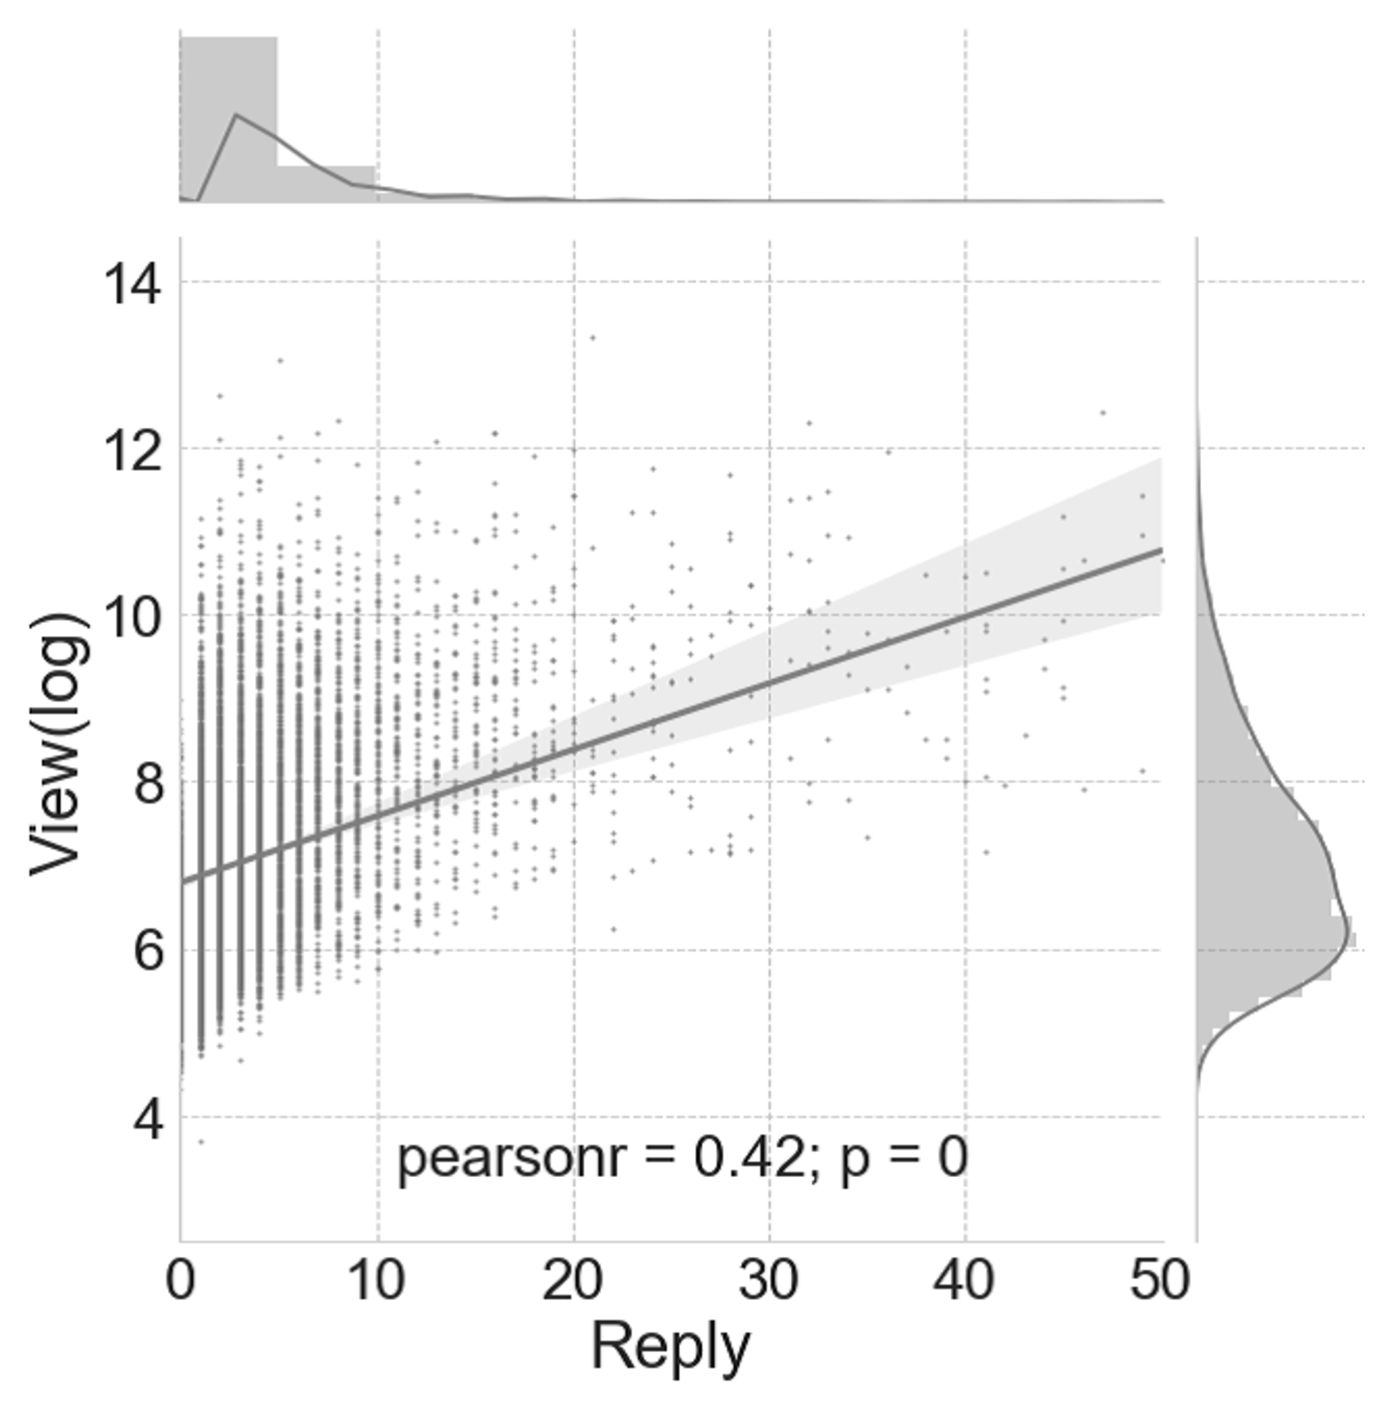
\includegraphics[width=6cm]{./eps/jointplot_view_reply.eps}
    \caption{閲覧数と返信数(1)}
    \label{fig:graf_view_reply_community1}
  \end{center}
  \begin{center}
    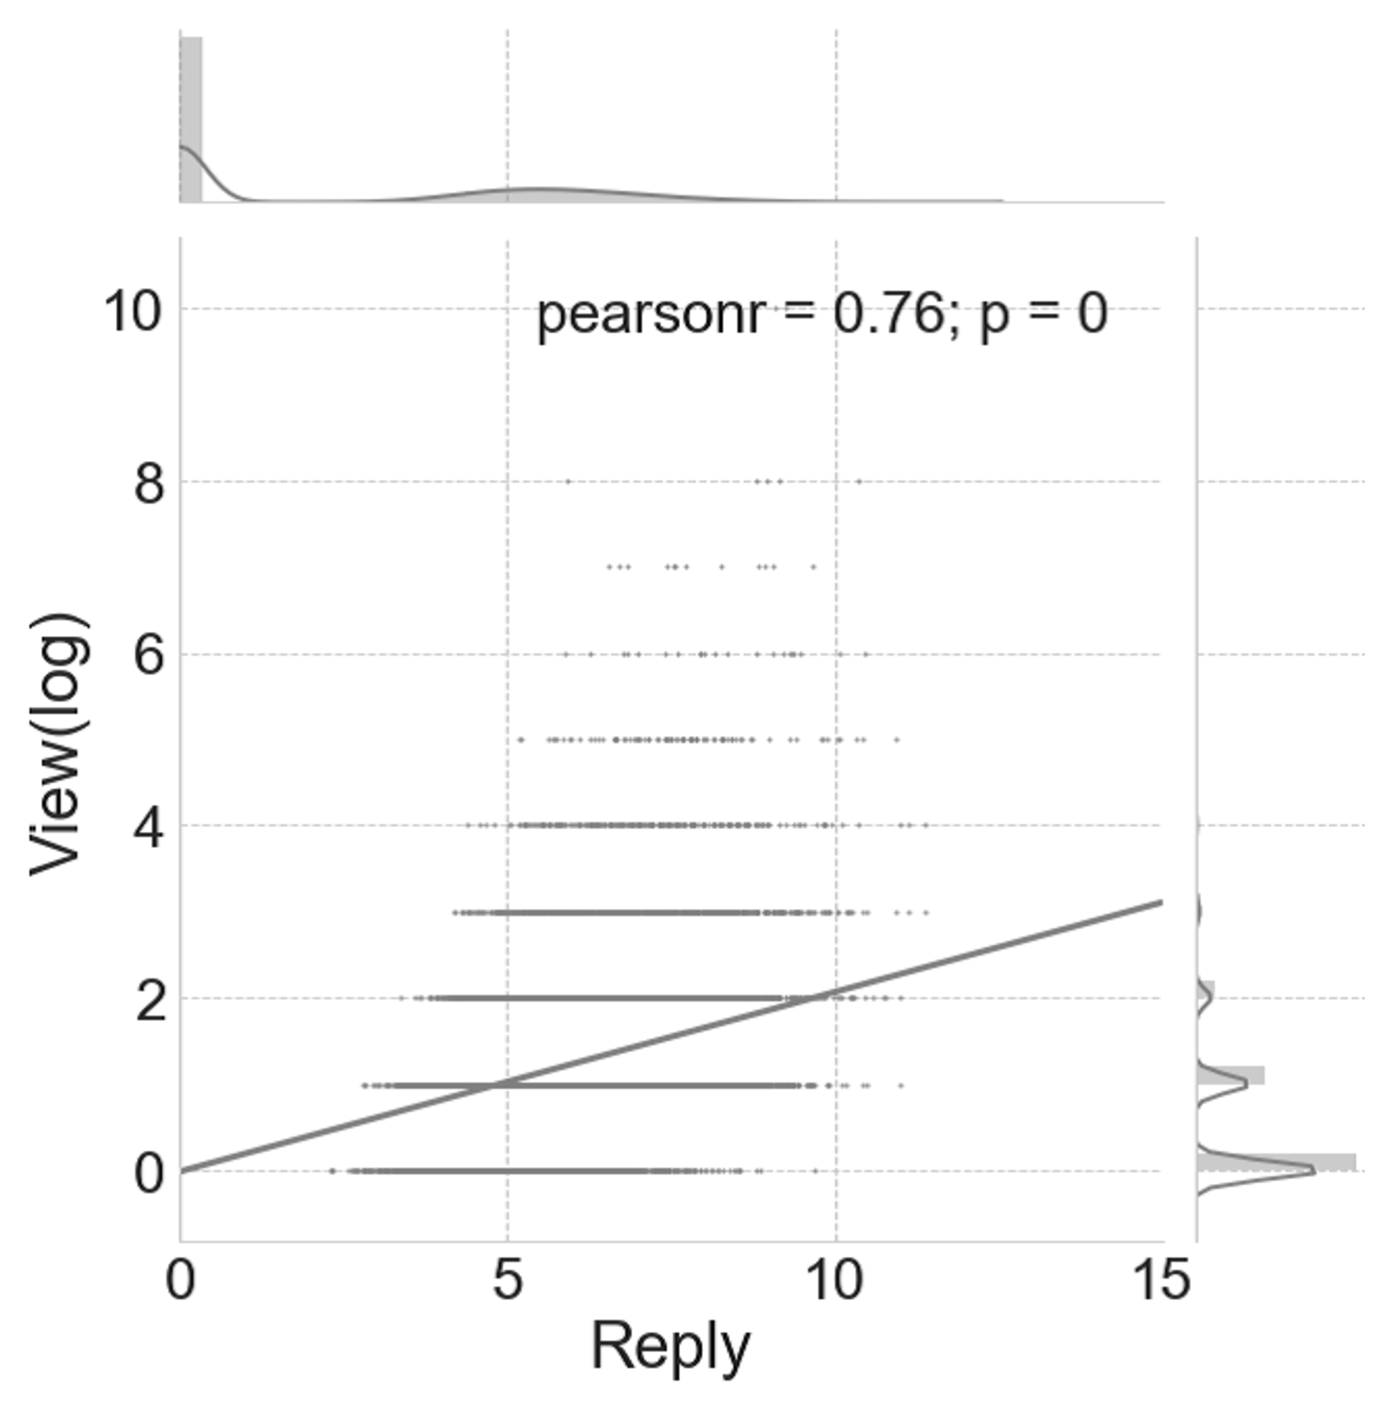
\includegraphics[width=6cm]{./eps/jointplot_view_reply_stackoverflow.eps}
    \caption{閲覧数と返信数(2)}
    \label{fig:graf_view_reply_stackoverflow}
  \end{center}
\end{figure}


図\ref{fig:graf_view_reply_community1}では,
質問記事の閲覧数は正規分布の傾向が確認できた.
%
返信数は返信がない質問記事も多い一方で,
質問記事の1件に対し,
40件から50件程の返信がある場合もある.
%
したがって,オンラインコミュニティ1は閲覧に対し,
返信のバリエーションが多いコミュニティであると言える.
閲覧数に対する返信数の相関係数は,$0.42$を示した.

図\ref{fig:graf_view_reply_stackoverflow}では,
閲覧数が少ない質問記事が多い一方で,
閲覧された質問記事に対しては,返信される傾向がある.
%
したがって,オンラインコミュニティ2は閲覧に対し,
均質な返信が行われるコミュニティであると言える.
閲覧数に対する返信数の相関係数は,$0.76$という高い相関が明らかになった.


結果,2種類のオンラインコミュニティで閲覧数と返信数には相関があり,
閲覧数はコミュニティのコミュニケーションを増加させる要素であることが明らかになった.
%
このため,話題性の多寡を評価する基準に閲覧数を用いることは妥当であると言える.

%5.1
\subsection{オンラインコミュニティ1への適用}\label{result_1}
オンラインコミュニティ1に対して,
NMFの基底数を$M=50$に設定し,
提案手法の適用を行った.
%
提案手法による基底の評価結果を図\ref{fig:graf_factor_result1}に示す.
%
\begin{figure}[htb]
  \begin{center}
    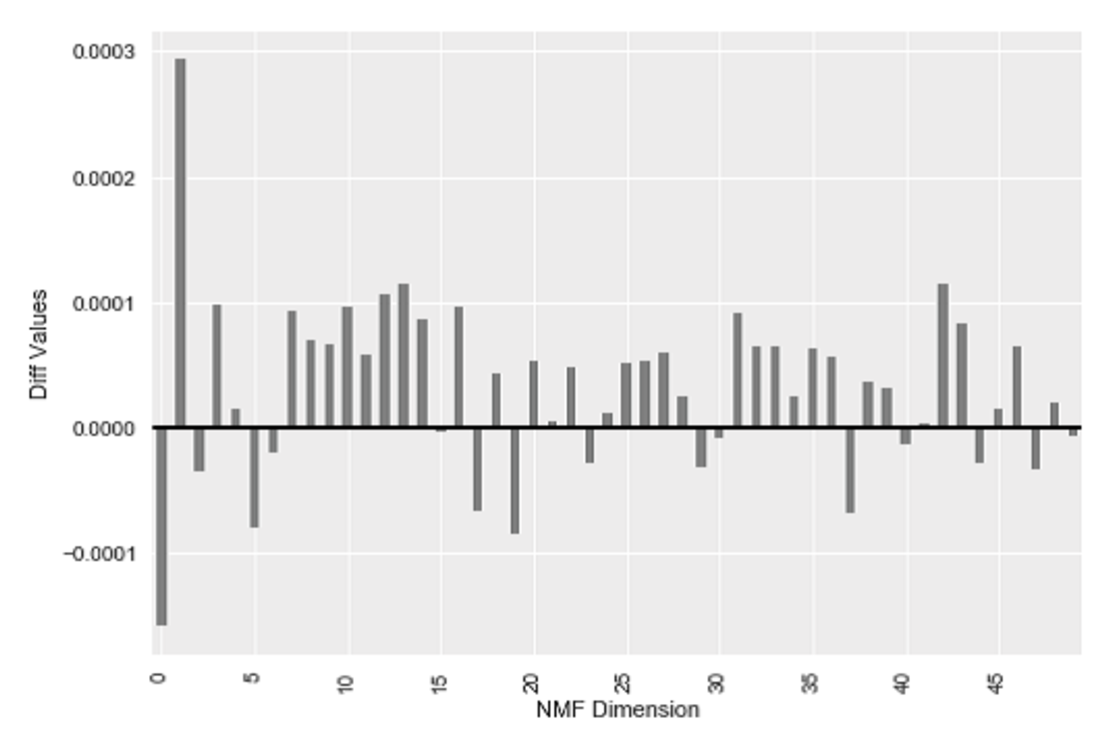
\includegraphics[width=7cm]{./eps/u_histgram_diff.eps}
    \caption{閲覧数に寄与率が高い基底}
    \label{fig:graf_factor_result1}
  \end{center}
\end{figure}

図\ref{fig:graf_factor_result1}の横軸が
基底$m$の特性を表す集合$S_{m}$の要素である.
また,縦軸が集合間における係数の平均値の差である.
%
縦軸の値が非負値の基底が,
閲覧数が平均値以上のベクトル集合である
$L_{1}$の特性を表す基底である.
%
結果,基底1が非負値で最も差異が大きいと評価された.
したがって,基底1が閲覧数が平均値以上の
集合$L_{1}$の特性を表す基底である.

得られた結果の基底1を基底選択して,
SVRを用いて回帰分析を行い,閲覧数の予測を行い,
予測誤差であるMAEを算出した結果を
図\ref{fig:graf_mae100-2000}および図\ref{fig:graf_mae25-400}に示す.

また同様に,RMSEを算出した結果を
図\ref{fig:graf_rmse100-2000}および図\ref{fig:graf_rmse25-400}に示す.
%
図のInput Featureは,回帰分析で用いる際の特徴量の数である.
回帰分析の特徴量は,基底1に対する寄与率の順に用いている.

\begin{figure}[htb]
  \begin{center}
    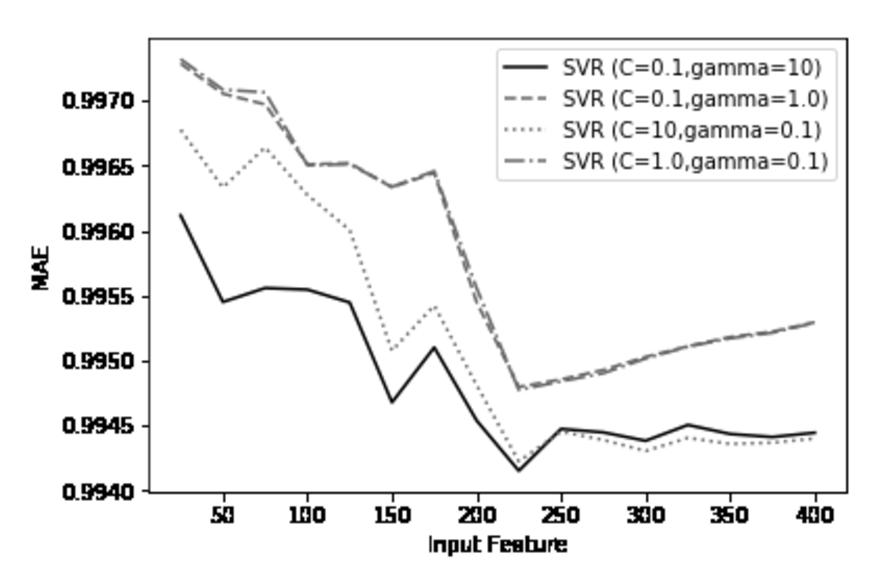
\includegraphics[width=6.5cm]{./eps/mae_svr_25-400.eps}
    \caption{回帰分析の結果を用いたMAE(1)}
    \label{fig:graf_mae25-400}
  \end{center}
\end{figure}
%
\begin{figure}[htb]
  \begin{center}
    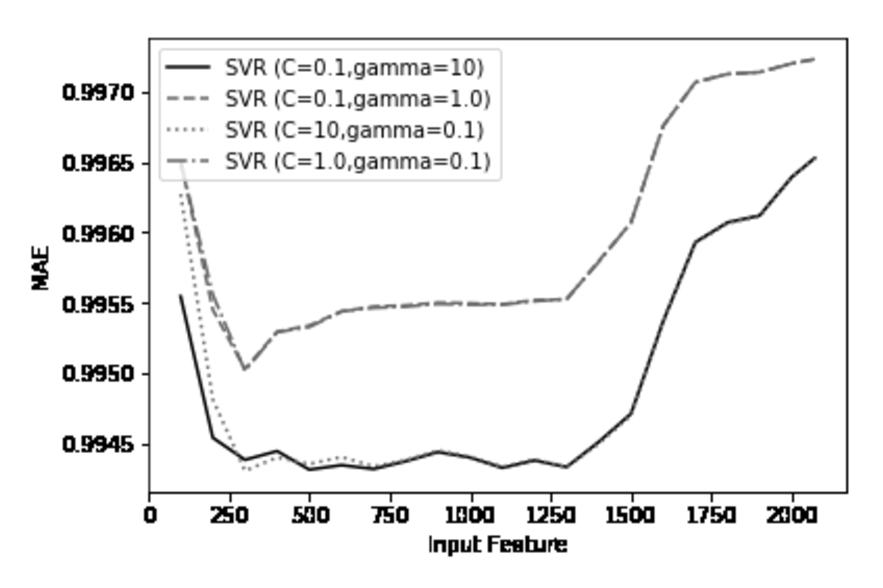
\includegraphics[width=6.5cm]{./eps/mae_svr_100-2000.eps}
    \caption{回帰分析の結果を用いたMAE(2)}
    \label{fig:graf_mae100-2000}
  \end{center}
\end{figure}
%
\begin{figure}[htb]
  \begin{center}
    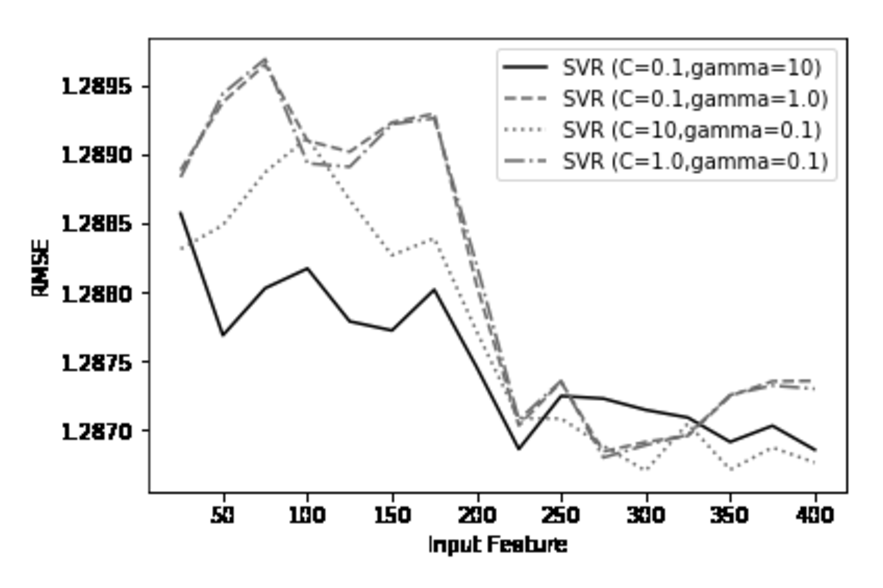
\includegraphics[width=6.5cm]{./eps/rmse_svr_25-400.eps}
    \caption{特徴選択数と回帰分析のRMSE(1)}
    \label{fig:graf_rmse25-400}
  \end{center}
\end{figure}

\newpage
\begin{figure}[htb]
  \begin{center}
    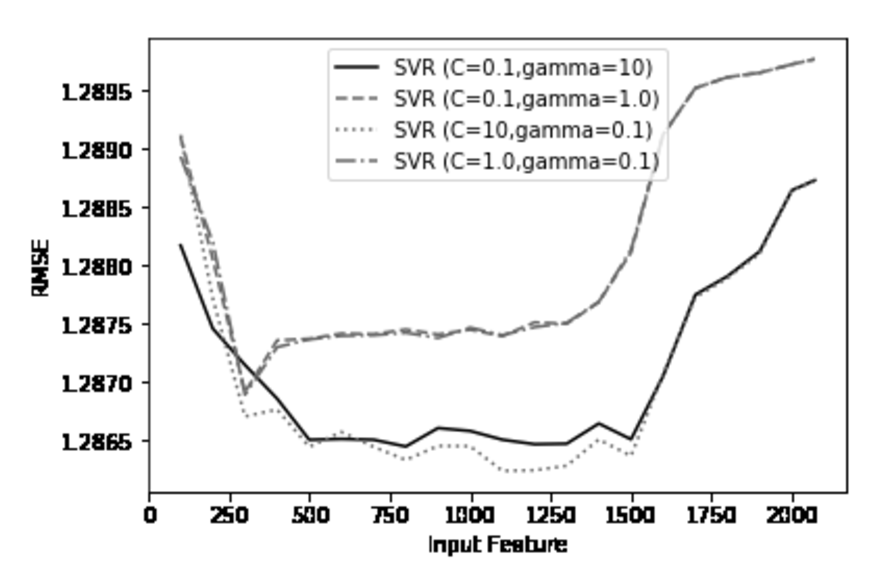
\includegraphics[width=6.5cm]{./eps/rmse_svr_100-2000.eps}
    \caption{特徴選択数と回帰分析のRMSE(2)}
    \label{fig:graf_rmse100-2000}
  \end{center}
\end{figure}

MAEの場合,
入力特徴選択数が250個前後が最も精度が良い(図\ref{fig:graf_mae25-400}).
一方で,1250-1500個以上の入力特徴量がある場合,
精度が下がる(図\ref{fig:graf_mae100-2000}).
%
結果,すべての特徴量を用いた場合よりも,
提案手法で得られた基底1に寄与率の高い少数の特徴量を
特徴選択した場合の方が,精度が高い.
%
RMSEの場合,
入力特徴選択数が200-250個が最も精度が良い(図\ref{fig:graf_rmse25-400}).
一方で,1500個以上の入力特徴量がある場合,精度が下がる(図\ref{fig:graf_rmse100-2000}).
%
結果,MAEと同様に,すべての特徴量を用いた場合よりも,
提案手法で得られた基底1に寄与率の高い少数の特徴量を
特徴選択した場合の方が,精度が高い.
%
したがって,MAEおよびRMSEを用いた,非線形回帰において,
基底選択に基づ特徴量の選択は妥当であることがデータで示された.
%
最後に,基底1に対する特徴量の
寄与率上位の10個を表\ref{tab:nmf_h1_view}に示す.
%
\begin{table}[htb]
  \caption{基底1の寄与率上位10個の特徴量}
  \label{tab:nmf_h1_view}
  \begin{center}
  \begin{tabular}{|c|c|c|c|} \hline
    & 特徴量名 & & 特徴量名 \\ \hline \hline
    1 & 固有(一般) & 6 & 機能(I-目的) \\ \hline
    2 & 機能(I-順接仮定)  & 7 & ひらがな(頻度) \\ \hline
    3 & 品詞(助詞)  & 8 & 機能(I-不可能) \\ \hline
    4 & 意味(2)(4.112)  & 9 & 機能(I-依頼) \\ \hline
    5 & 機能(I-様態)  & 10 & 機能(B-自然発生) \\ \hline
  \end{tabular}
  \end{center}
\end{table}

表\ref{tab:nmf_h1_view}の「固有(一般) 」は「固有名詞」,
「機能(*)」は「機能表現タグ」,「意味」は「意味分類コード」である.
%
意味分類コード(2)(4.112)の単語は,
「その他の類(展開)」の「ですから」「まして」「だから」などである.
%
結果,選択基底は,固有名詞やひらがなの頻度の寄与が高く,
機能表現タグの寄与が多い,基底であることが明らかになった.

\newpage
%5.2
\subsection{オンラインコミュニティ1の文書分類}\label{result_2}
オンラインコミュニティ1より得られた特徴量を用いて
文書分類実験を行った結果を
表\ref{tab:nmf_class_all}から表\ref{tab:nmf_class_related2}に示す.

\begin{table}[htb]
  \caption{全特徴量} 
  \label{tab:nmf_class_all}
  \begin{center}
  \begin{tabular}{c|c|c|c} \hline
    分類器 & 適合率 & 再現率 & F値 \\ \hline \hline
  AdaBoost & 0.45 & 0.29 & 0.35 \\ \hline
  RandomForest & 0.44 & 0.26 & 0.33 \\ \hline
  MLP & 0.00 & 0.00 & 0.00 \\ \hline
  K-NN & 0.42 & 0.37 & 0.39 \\ \hline
  \end{tabular}
  \end{center}
\end{table}
%
\begin{table}[htb]
  \caption{特徴量選択(提案手法 基底の寄与率)} 
  \label{tab:nmf_class_proposed}
  \begin{center}
  \begin{tabular}{c|c|c|c} \hline
    分類器 & 適合率 & 再現率 & F値 \\ \hline \hline
  AdaBoost & 0.43 & 0.23 & 0.30 \\ \hline
  RandomForest & 0.45 & 0.29 & 0.35 \\ \hline
  MLP & 0.40 & 0.04 & 0.08 \\ \hline
  K-NN & 0.44 & 0.42 & 0.43 \\ \hline
  \end{tabular}
  \end{center}
\end{table}
%
\begin{table}[htb]
  \caption{特徴量選択(単変量特徴量選択)} 
  \label{tab:nmf_class_related1}
  \begin{center}
  \begin{tabular}{c|c|c|c} \hline
    分類器 & 適合率 & 再現率 & F値 \\ \hline \hline
  AdaBoost & 0.46 & 0.28 & 0.35 \\ \hline
  RandomForest & 0.45 & 0.28 & 0.34 \\ \hline
  MLP & 0.00 & 0.00 & 0.00 \\ \hline
  K-NN & 0.42 & 0.38 & 0.40 \\ \hline
  \end{tabular}
  \end{center}
\end{table}
%
\begin{table}[htb]
  \caption{特徴量選択(再帰的特徴量削減)} 
  \label{tab:nmf_class_related2}
  \begin{center}
  \begin{tabular}{c|c|c|c} \hline
    分類器 & 適合率 & 再現率 & F値 \\ \hline \hline
  AdaBoost & 0.44 & 0.29 & 0.35 \\ \hline
  RandomForest & 0.45 & 0.27 & 0.34 \\ \hline
  MLP & 0.00 & 0.00 & 0.00 \\ \hline
  K-NN & 0.43 & 0.38 & 0.40 \\ \hline
  \end{tabular}
  \end{center}
\end{table}

表\ref{tab:nmf_class_all}は,得られたすべての特徴量を用いて,
文書分類した結果である.
%
表\ref{tab:nmf_class_proposed}が,
提案手法で得られた基底1の寄与率上位100個の特徴量を特徴選択し,
文書分類した結果である.
%
表\ref{tab:nmf_class_related1}は,
既存手法である単変量特徴量選択を用いて特徴量選択した結果であり,
%
表\ref{tab:nmf_class_related2}は,
既存手法である再帰的特徴量削減を用いて特徴量選択し,
文書分類した結果である.
%
すべての特徴量およびいずれの特徴量選択を用いた場合でも,
オンラインコミュニティ1の質問記事では,特徴量選択手法に関わらず,
文書分類の精度は十分ではない.

結果から,提案手法ではなく,
閲覧数の平均値を基に行った文書分類のラベリングの
評価基準が妥当ではなかったと判断できる.
%\newpage

%5.3
\subsection{オンラインコミュニティ2への適用}\label{result_3}
評価では,NMFの基底数を$M=50$に設定し,提案手法の評価を行った.
提案手法による基底選択の結果を図\ref{fig:graf_factor}に示す.
%
\begin{figure}[htb]
  \begin{center}
    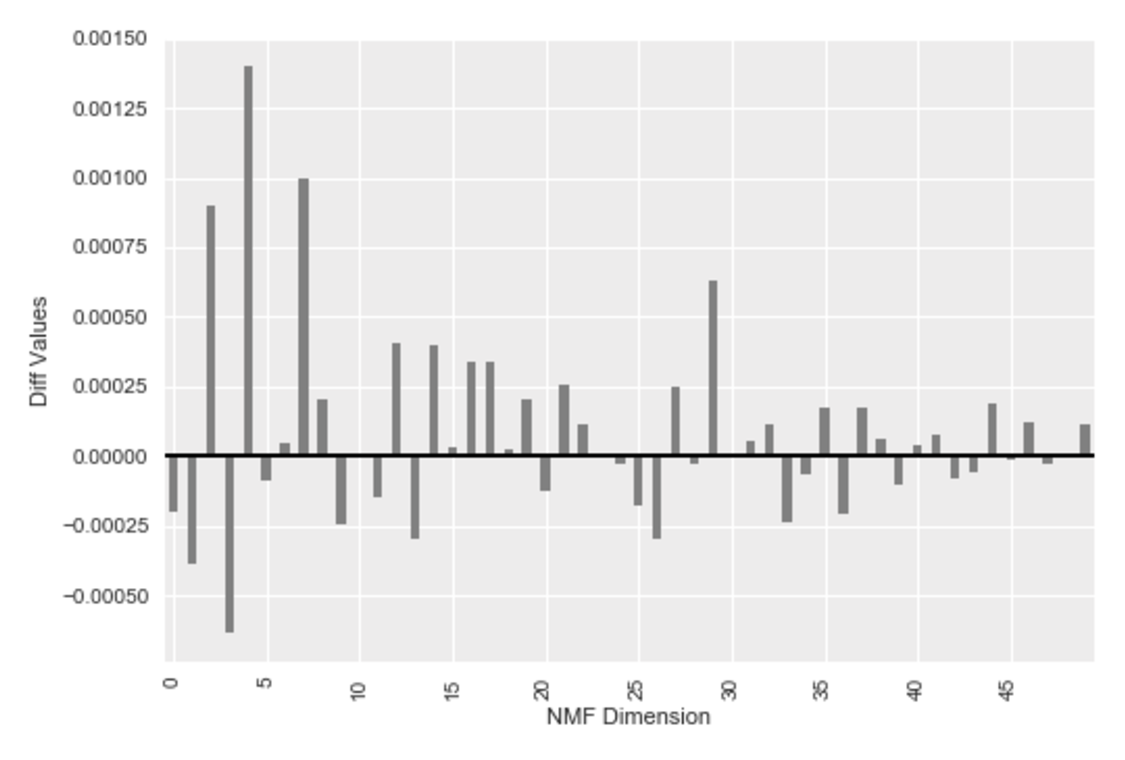
\includegraphics[width=7.8cm]{./eps/u_histgram_diff_stackoverflow.eps}
    \caption{閲覧数に寄与率が高い特徴量と状況変数}
    \label{fig:graf_factor}
  \end{center}
\end{figure}

NMF の基底数をM = 50 に設定し,提案手法の評価を行った.
横軸が基底m の特性を表す集合Sm の要素である.
また,縦軸が集合間における係数の平均値の差である.
縦軸の値が非負値の基底が,
閲覧数が平均値以上のベクトル集合であるL1 の特性を表す基底である.
追加実験では,基底4 が非負値で最も差異が大きいと評価された.

基底4を用いて,
SVRを用いて回帰分析を行い,閲覧数の予測を行い,
予測誤差であるMAEを算出した結果を
図\ref{fig:graf_mae100-2000_stackoverflow}および図\ref{fig:graf_mae25-400_stackoverflow}に示す.
%
また同様に,RMSEを算出した結果を
図\ref{fig:graf_rmse100-2000_stackoverflow}および図\ref{fig:graf_rmse25-400_stackoverflow}に示す.

\begin{figure}[htb]
  \begin{center}
    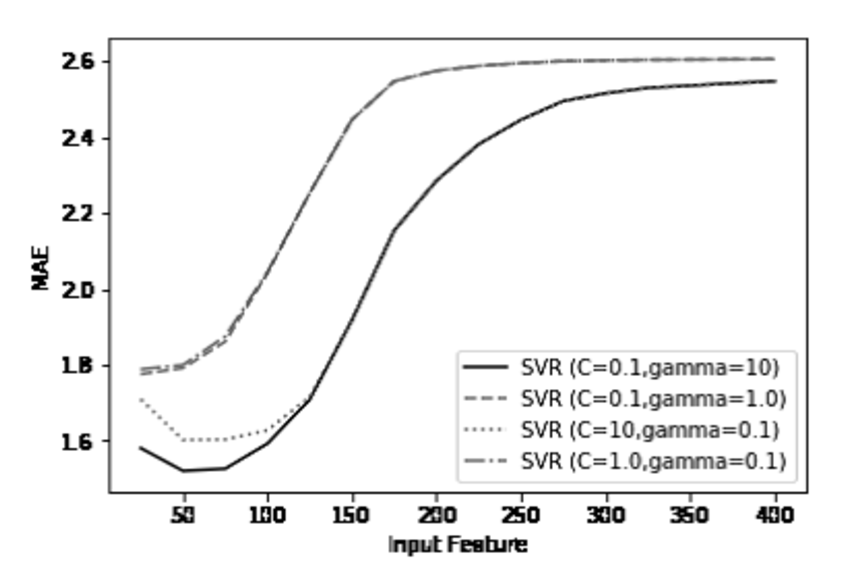
\includegraphics[width=6.5cm]{./eps/Regression-MAE-RBF_25-400.eps}
    \caption{回帰分析の結果を用いたMAE(1)}
    \label{fig:graf_mae25-400_stackoverflow}
  \end{center}
\end{figure}

\newpage
\begin{figure}[htb]
  \begin{center}
    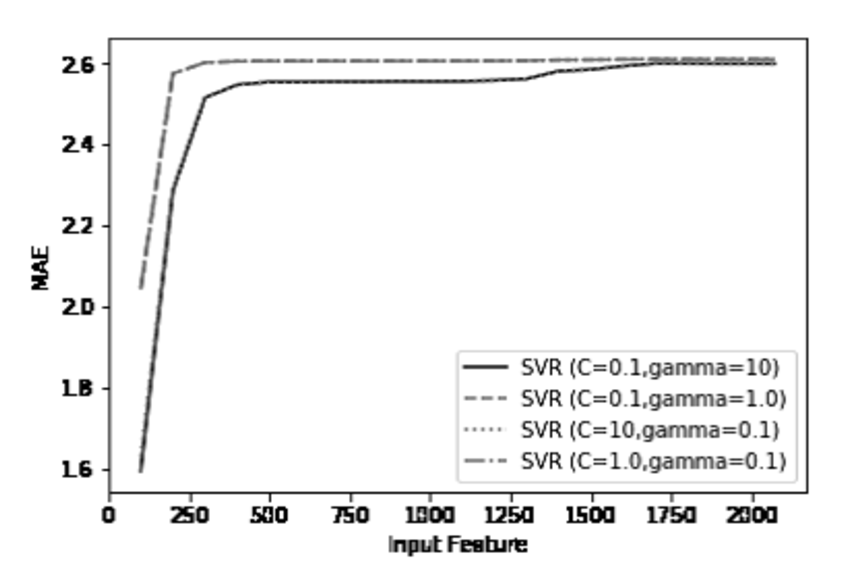
\includegraphics[width=6.5cm]{./eps/Regression-MAE-RBF_2071.eps}
    \caption{回帰分析の結果を用いたMAE(2)}
    \label{fig:graf_mae100-2000_stackoverflow}
  \end{center}
\end{figure}
%
図のInput Featureは,回帰分析で用いる際の特徴量の数である.
また,回帰分析の特徴量は,基底4に対する寄与率の順に用いている.
%
MAEの場合,
入力特徴選択数が50-100個前後が最も精度が良い(図\ref{fig:graf_mae25-400_stackoverflow}).
一方で,100個以上の入力特徴量がある場合,精度が下がる(図\ref{fig:graf_mae100-2000_stackoverflow}).
%
入力特徴選択数が50個である場合と250個以上である場合は,
予測精度の差は明らかである.
%
結果,すべての特徴量を用いた場合よりも,
提案手法で得られた基底4に寄与率の高い少数の特徴量を
特徴選択した場合の方が,精度が高い.

RMSEの場合,入力特徴選択数が50-100個が最も精度が良い(図\ref{fig:graf_rmse25-400_stackoverflow}).
入力特徴選択数が50個である場合と250個以上である場合は,
予測精度の差は明らかである(図\ref{fig:graf_rmse100-2000_stackoverflow}).
%
結果,すべての特徴量を用いた場合よりも,
提案手法で得られた基底4に寄与率の高い少数の特徴量を
特徴選択した場合の方が,回帰分析の予測精度が高い.
%
したがって,MAEおよびRMSEを用いた,非線形回帰において,
基底選択に基づく寄与率による特徴量の選択は妥当であり,
有効であることがデータで示された.
\newpage

\begin{figure}[htb]
  \begin{center}
    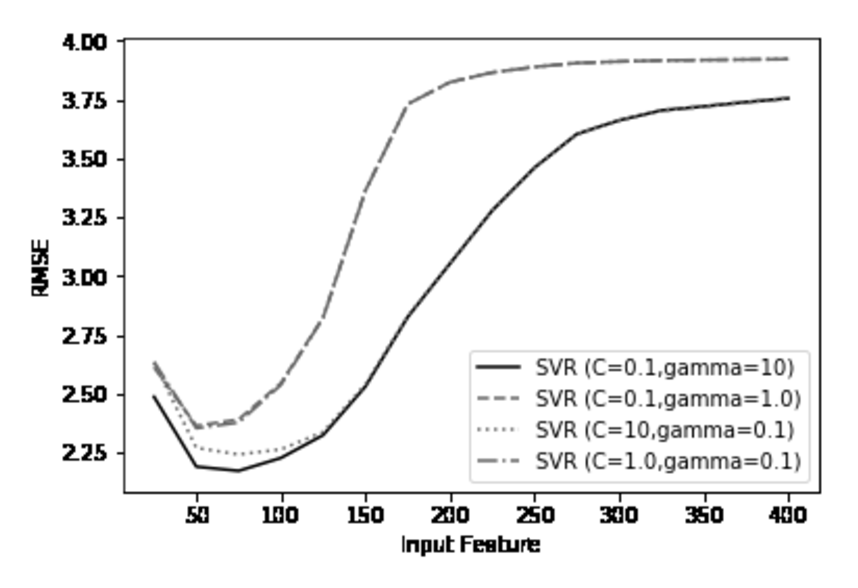
\includegraphics[width=6.5cm]{./eps/Regression-RMSE-RBF_25-400.eps}
    \caption{特徴選択数と回帰分析のRMSE(1)}
    \label{fig:graf_rmse25-400_stackoverflow}
  \end{center}
\end{figure}
%
\begin{figure}[htb]
  \begin{center}
    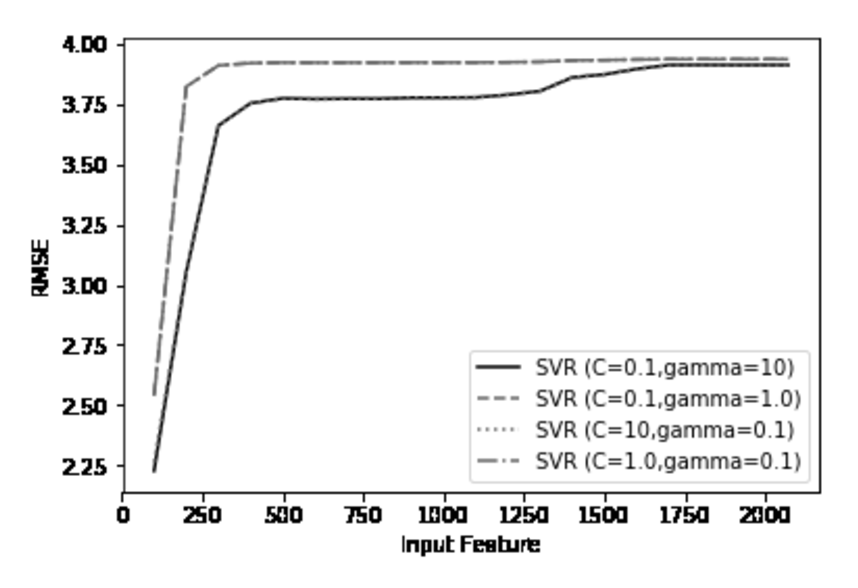
\includegraphics[width=6.5cm]{./eps/Regression-RMSE-RBF_2071.eps}
    \caption{特徴選択数と回帰分析のRMSE(2)}
    \label{fig:graf_rmse100-2000_stackoverflow}
  \end{center}
\end{figure}

最後に,基底4に対する特徴量の
寄与率上位の10個を表\ref{tab:nmf_h4_view}に示す.
\begin{table}[htb]
  \caption{基底4の寄与率上位10個の特徴量}
  \label{tab:nmf_h4_view}
  \begin{center}
  \begin{tabular}{|c|c|c|c|} \hline
    & 特徴量名 & & 辞書の単語 \\ \hline \hline
    1 & TOPIC(LDA) & 6 & 意味(2)(1.353) \\ \hline
    2 & 意味(2)(2.304) & 7 & 意味(2)(4.35) \\ \hline
    3 & 意味(2)(1.304) & 8 & 意味(2)(1.564) \\ \hline
    4 & 意味(2)(1.366) & 9 & 意味(2)(3.133) \\ \hline
    5 & 意味(2)(4.314) & 10 & TOPIC(LDA) \\ \hline
  \end{tabular}
  \end{center}
\end{table}

表\ref{tab:nmf_h4_view}の「意味」は「意味分類コード」である.
結果,基底4は,意味分類コードの寄与が高い基底である.
意味分類コードは語を意味に基づいて分類した語彙表による特徴量である.
語彙は,ある言語体系,地域,分野などで用いられる語の総体であり,
意味とは,言葉や記号などで表現され,理解される一定の内容である.
ゆえに,理解されやすい特徴量の寄与が高い基底であることが明らかになった.

\newpage
%5.4
\subsection{オンラインコミュニティ2の文書分類}\label{result_4}
オンラインコミュニティ2より得られた特徴量を用いて
文書分類実験を行った結果を
表\ref{tab:nmf_class_all_stackoverflow}から表\ref{tab:nmf_class_related2_stackoverflow}に示す.

\begin{table}[htb]
  \caption{全特徴量} 
  \label{tab:nmf_class_all_stackoverflow}
  \begin{center}
  \begin{tabular}{c|c|c|c} \hline
    分類器 & 適合率 & 再現率 & F値 \\ \hline \hline
  AdaBoost & 0.89 & 0.87 & 0.88 \\ \hline
  RandomForest & 0.87 & 0.78 & 0.82 \\ \hline
  MLP & 0.92 & 0.88 & 0.90 \\ \hline
  K-NN & 0.83 & 0.75 & 0.78 \\ \hline
  \end{tabular}
  \end{center}
\end{table}
%\newpage

\begin{table}[htb]
  \caption{特徴量選択(提案手法 基底の寄与率)} 
  \label{tab:nmf_class_proposed_stackoverflow}
  \begin{center}
  \begin{tabular}{c|c|c|c} \hline
    分類器 & 適合率 & 再現率 & F値 \\ \hline \hline
  AdaBoost & 0.87 & 0.83 & 0.85 \\ \hline
  RandomForest & 0.87 & 0.82 & 0.84 \\ \hline
  MLP & 0.87 & 0.87 & 0.87 \\ \hline
  K-NN & 0.85 & 0.80 & 0.83 \\ \hline
  \end{tabular}
  \end{center}
\end{table}
%
\begin{table}[htb]
  \caption{特徴量選択(単変量特徴量選択)} 
  \label{tab:nmf_class_related1_stackoverflow}
  \begin{center}
  \begin{tabular}{c|c|c|c} \hline
    分類器 & 適合率 & 再現率 & F値 \\ \hline \hline
  AdaBoost & 0.88 & 0.85 & 0.87 \\ \hline
  RandomForest & 0.88 & 0.83 & 0.85 \\ \hline
  MLP & 0.00 & 0.00 & 0.00 \\ \hline
  K-NN & 0.87 & 0.83 & 0.85 \\ \hline
  \end{tabular}
  \end{center}
\end{table}
%
\begin{table}[htb]
  \caption{特徴量選択(再帰的特徴量削減)} 
  \label{tab:nmf_class_related2_stackoverflow}
  \begin{center}
  \begin{tabular}{c|c|c|c} \hline
    分類器 & 適合率 & 再現率 & F値 \\ \hline \hline
  AdaBoost & 0.89 & 0.86 & 0.87 \\ \hline
  RandomForest & 0.88 & 0.84 & 0.86  \\ \hline
  MLP & 0.00 & 0.00 & 0.00  \\ \hline
  K-NN & 0.88 & 0.82 & 0.85  \\ \hline
  \end{tabular}
  \end{center}
\end{table}

表\ref{tab:nmf_class_all_stackoverflow}は,得られたすべての特徴量を用いて,
文書分類した結果である.
%
表\ref{tab:nmf_class_proposed_stackoverflow}が,
提案手法で得られた基底1の寄与率上位100個の特徴量を特徴選択し,
文書分類した結果である.
%
表\ref{tab:nmf_class_related1_stackoverflow}は,
既存手法である単変量特徴量選択を用いて特徴量選択した結果であり,
%
表\ref{tab:nmf_class_related2_stackoverflow}は,
既存手法である再帰的特徴量削減を用いて特徴量選択し,
文書分類した結果である.
%
結果,オンラインコミュニティ2では,
正解クラスへの分類結果は$0.8$以上の高い分類精度が得られた.

\newpage
したがって,提案手法で得られた特徴量は,
文書分類に有効であることが明らかである.
%
加えて,オンラインコミュニティ2においては,
閲覧数の平均値を基に行った文書分類のラベリングの
評価基準が妥当であることが明らかになった.

%6
\section{考察}
%6.1
\subsection{話題性の予測}
評価に用いたオンラインコミュニティの考察から,始める.
%
まず,オンラインコミュニティ1は,Appleサポートコミュニティのデータセットである.
%
Appleサポートコミュニティは,
コンシューマ\footnote{
商品やサービスの最終的な利用者,消費者のこと.
消費者という概念はある商品やサービスを直接利用する人であるが,
購買行為を決定する人も含めて消費者と呼ぶこともある
\cite{book_media}.
}が,直接質問記事を投稿する.
また,利用者層の幅は非常に広い.
%
したがって,メディアとして考察した場合は,
ゼネラル・メディア
\footnote{
年齢,教育程度,職業,ライフスタイルなど,あらゆる社会層の人々を普遍的にオーディエンスとしている媒体.
マス・メディアをオーディエンスの態様から分類した概念.一般日刊紙やテレビなど\cite{book_media}.
}
に相当する性質を持つ.

一方で,オンラインコミュニティ2は,stackover flowのデータセットである.
stack overflowはStack ExchangeのQ\&Aコミュニティの一つであり
開発者向けのコミュニティである.
stack overflowは専門家や熟練者など,高度な知識を持つ,エキスパートが利用者である.
このため,メディアとして考察した場合は,
クラス・メディア\footnote{
特定の社会層もしくは集団を対象にした媒体.雑誌やラジオなど\cite{book_media}.
また,業界誌や専門雑誌,ダイレクト・メールなど限定された対象を相手にする媒体も含まれる.}に近い性質を持つ.

\ref{result_1}節の結果から,各オンラインコミュニティで,
閲覧数と経過日数の相関係数が大きく異なることが明らかになった.
%
また,閲覧数と返信数の相関係数においても,
オンラインコミュニティ1で$0.42$,オンラインコミュニティ2で$0.76$である.

\newpage
ゆえに,質問記事を閲覧した際の返信度合いは,
オンラインコミュニティのメディアの性質で異なると推定される.

ここで,オンラインコミュニティの一つである
不満買取センター
\footnote{
不満買取センター : http://fumankaitori.com
}
の不満カテゴリ辞書データを用いて,
オンラインコミュニティのコンテンツを考察する.
%
不満カテゴリ辞書は,2015年3月18日から,2016年12月1日までのノイズを排除した
投稿記事3,527,336件から作成されている\cite{insight_tech}.
辞書のエントリ数は953,776件であり,
複数カテゴリに登録されている重複エントリを除いたエントリ数は110,866件である.
%
不満買取センターに不満投稿が投稿されるカテゴリと,
特徴的な単語の例を表\ref{tab:insight_tec_dataset}に示す.
%
単語は,不満カテゴリ辞書のTF-IDF
\footnote{
単語の重み付け技法の一つ.
文書内単語の相対的な重要性を表す正規化されたスコア.
単語の頻度と文書頻度の逆数で算出.
}
におけるスコア上位エントリの名詞である.

\begin{table}[htb]
  \caption{不満買取センターのカテゴリと単語の例\cite{insight_tech}}
  \label{tab:insight_tec_dataset}
  \begin{center}
  \begin{tabular}{c|c} \hline
    カテゴリ名 & 単語の例 \\ \hline \hline
  暮らし・住まい & 布団,雨,枕 \\ \hline
  ファッション & 腕時計,靴 \\ \hline
  趣味・エンタメ & 映画,CD \\ \hline
  食品・飲料 & グミ,ワイン \\ \hline
  外食・店舗 & 弁当,居酒屋 \\ \hline
  医療・福祉 & 整体,介護,薬 \\ \hline
  アウトドア・スポーツ & バイク,自転車 \\ \hline
  デジタル・家電 & 録画,デジカメ \\ \hline
  宿泊・観光・レジャー & ホテル,部屋 \\ \hline
  公共・環境 & バス,飛行機 \\ \hline
  教育 & 幼稚園,保育園 \\ \hline
  国際・文化 & 留学,日本 \\ \hline
  政治・行政 & 選挙,政治家 \\ \hline
  人間関係 & 離婚,結婚,人 \\ \hline
  仕事 &  転職,仕事,面接 \\ \hline
  ペット &  ペットショップ \\ \hline
  \end{tabular}
  \end{center}
\end{table}

ところで,不満カテゴリ辞書データの特徴的な単語は,
登録カテゴリで異なる.
%
また辞書では,飲食物の商品名など,
商品の固有名詞も登録されており,
商品名は食品・飲料や,宿泊・観光・レジャーなど,
関連性のある複数カテゴリで登録されている.

\newpage
一方で,他のカテゴリで登録されている特徴的な単語であっても,
関連性がないカテゴリでは登録されていない.

結果から,不満買取センターにおける不満投稿では,
関連性がないカテゴリでは単語の登録がないことが明らかになった.
%
カテゴリにおいて,特徴的な単語が異なることは,
各カテゴリが,異なるメディアあるいは,コミュニティであると言える.
%
ゆえに,コンテンツが広範なゼネラル・メディアの
オンラインコミュニティの場合,
オンラインコミュニティの各カテゴリが,
クラス・メディアに相当すると推定される.
%
したがって,同一のオンラインコミュニティであっても,
メディアの性質で異なると推定される.
%
評価実験の話題性の予測では,
オンラインコミュニティ1およびオンラインコミュニティ2で,
特徴量選択は予測誤差の精度は有効な結果であった.
%.
しかし,オンラインコミュニティ2の予測精度の向上は明らかである一方で,
オンラインコミュニティ1の予測精度の向上は限定的であった.
%
\ref{result_1}節の結果から,
オンラインコミュニティ1は,ゼネラル・メディアに相当すると推定される.
ゼネラル・メディアの性質を持つオンラインコミュニティの場合,
コンテンツの広範であり,カテゴリが多い.
したがって,表\ref{tab:insight_tec_dataset}のように,
カテゴリが異なった場合,特徴的な単語は異なると推定される.
%\newpage

本研究で用いたトピックモデルアルゴリズムは,
カテゴリ分類においても有効なアルゴリズムである.
%
提案手法の適用の結果,オンラインコミュニティ1では,
閲覧数予測においては,有効性は限定的であった.
%
ゼネラル・メディアに近い性質を持つオンラインコミュニティ1は,利用者が広範である.
したがって,閲覧数が増加しやすい傾向や特徴的な単語が不明瞭であることなどが推定される.
%
このため,オンラインコミュニティ1の閲覧数予測の精度向上には,
カテゴリ分類後に,閲覧数予測を行う必要があると推定される.

一方で,オンラインコミュニティ2は\ref{result_1}節の結果から,
クラス・メディアの性質を持つと推定される.
オンラインコミュニティ2はオンラインコミュニティ1と比較して,
利用者が限られた範囲である.
%
提案手法の適用の結果,オンラインコミュニティ2では,
閲覧数予測において,高い有効性が明らかになった.
%
これは,クラス・メディアの性質を持つオンラインコミュニティ2は,
利用者が限られており,閲覧数が増加しやすい一定の傾向が存在することや,
あるいは閲覧数が増加する特徴的な単語が明瞭であることなどが要因であると推定される.
%
加えて,コンテンツも限られた範囲であり,
カテゴリが異なった場合でも,
特徴的な単語は類似の傾向があると推定される.

ゆえに,SVRで回帰分析を行った際に,
クラス・メディアであるオンラインコミュニティ2は明瞭な結果となり,
ゼネラル・メディアであるオンラインコミュニティ1では
有効ではあるが限定的な結果であったと推定される.

%6.2
\subsection{話題性の判別}
%\begin{bfseries}
分類実験では,ゼネラル・メディアに相当するオンラインコミュニティ1と
クラス・メディアに相当するオンラインコミュニティ2で結果が大きく異なった.
%
まず,既存手法で抽出した特徴量を用いて,
文書分類を行った結果を考察する.

本研究の文書分類では,
質問記事の分類の基準となるラベルは,
閲覧数の平均値を基にラベリングした.
%
オンラインコミュニティ1の文書分類では,
すべての特徴量を用いた場合や,
既存研究の特徴量選択手法を用いた場合など,
いずれの手法を用いた場合でも,
正解クラスへの分類結果はF値で,$0.3$から$0.4$程度である.
パラメータの最適化を行わない場合,
MLPの分類器では分類困難である.

次に,オンラインコミュニティ1の層化5分割交差検証の
交差検証スコアを表\ref{tab:nmf_classifier_apple}に示す.
表\ref{tab:nmf_classifier_apple}のRFは,RandamForestsである.
%
\begin{table}[htb]
  \caption{交差検証(オンラインコミュニティ1)} 
  \label{tab:nmf_classifier_apple}
  \begin{center}
  \begin{tabular}{c|c|c|c|c|c} \hline
    分類器 & 1 & 2 & 3 & 4 & 5 \\ \hline \hline
    AdaBoost & 0.54 & 0.53 & 0.52 & 0.54 & 0.53 \\ \hline 
    RF & 0.52 & 0.54 & 0.53 & 0.52 & 0.52 \\ \hline 
    MLP & 0.55 & 0.55 & 0.56 & 0.54 & 0.55 \\ \hline 
    K-NN & 0.50 & 0.52 & 0.52 & 0.51 & 0.51 \\ \hline
  \end{tabular}
  \end{center}
\end{table}

表\ref{tab:nmf_classifier_apple}より,
交差検証スコアの場合でも,結果は十分ではない.
したがって,オンラインコミュニティ1では,
基底選択に関わらず,十分な文書分類が行えていないと言える.
%
このため,オンラインコミュニティ1では,
特徴量選択ではなく,
正解クラスのラベリング基準を最適値にする必要がある.

\newpage
一方で,オンラインコミュニティ2では,
既存研究の特徴量選択手法を用いた場合など,
いずれの手法を用いた場合でも,
正解クラスへの分類結果はF値で,
$0.7$から$0.9$の範囲である.

次に,オンラインコミュニティ1の層化5分割交差検証の
交差検証スコアを表\ref{tab:nmf_classifier_stackoverflow}に示す.
表\ref{tab:nmf_classifier_stackoverflow}のRFは,RandamForestsである.
%
\begin{table}[htb]
  \caption{交差検証(オンラインコミュニティ2)} 
  \label{tab:nmf_classifier_stackoverflow}
  \begin{center}
  \begin{tabular}{c|c|c|c|c|c} \hline
    分類器 & 1 & 2 & 3 & 4 & 5 \\ \hline \hline
    AdaBoost & 0.86 & 0.86 & 0.87 & 0.87 & 0.87 \\ \hline 
    RF & 0.86 & 0.85 & 0.87 & 0.86 & 0.87 \\ \hline 
    MLP & 0.89 & 0.88 & 0.89 & 0.89 & 0.90 \\ \hline 
    K-NN & 0.84 & 0.84 & 0.85 & 0.85 & 0.85 \\ \hline
  \end{tabular}
  \end{center}
\end{table}

表\ref{tab:nmf_classifier_apple}より,
交差検証スコアの場合でも,有効な結果であった.
したがって,オンラインコミュニティ2では,
閲覧数のラベリング基準は平均値が妥当であったことが明らかになった.

ここで,提案手法は,目的変数である閲覧数から,
有効な基底を明らかにし,基底選択を行う手法である.
%
文書分類で有効な結果が得られた
オンラインコミュニティ2の結果を用いて,
提案手法による基底選択の有効性を考察する.
%\newpage

基底選択の結果,基底の寄与率上位の特徴量で,
重要な特徴量が明らかになり,特徴量の評価が行える.
したがって,重要な特徴量のみを用いる特徴量選択が行える.
%
分類結果で考察した場合,
既存手法である単変量特徴量選択および再帰的特徴量削減では,
分類困難であったMLPによる分類が行えた.
%
したがって,分類器に依存せずに,少ない特徴量で,
すべての特徴量を用いた場合に相当する結果が得られた.
このため,分類器に依存せず有効な特徴量選択が行える手法である.

分類精度だが,提案手法を用いたと比較し,
すべての特徴量を用いた場合や,
既存手法の特徴量選択を行った場合の方が,
適合率や再現率,F値の結果は良い.
%
しかし一方で,値の差は誤差の範囲であり,
すべての特徴量を用いた場合と同程度の分類結果であり,
特徴量選択手法としての性能を有している.
加えて,既存の特徴量選択手法と,同程度の結果も得られた.

\newpage
特徴量選択としては,基底に対する特徴量の寄与率で,
統計的な関係を基にした単変量特徴量選択と同様に,
関係がないノイズに相当する特徴量の除去が行える.
%
また,計算量基準では,再帰的特徴量削減は,
特徴量の次元数を指定する場合,
特定の次元数になるまで,繰り返しモデルベースを適用する.
したがって,非常に大きな計算量を必要とする.
%
一方で,提案手法は基底を選択した場合に,
基底のベクトルである寄与率で特徴量を評価している.
%
したがって,計算量は,再帰的特徴量削減と比較して少ない.
このため,計算量基準では,既存手法である再帰的特徴量削減と比較し,
有効な特徴量選択である.
%
ゆえに,文書分類においては,提案手法は分類器に依存せず,
再帰的特徴量削減と比較して,
少ない計算量で特徴量選択が行える手法であると言える.

文書分類で有効な結果が得られたオンラインコミュニティ2で,
提案手法で得られた基底の特徴量を用いた結果の
Precision-recall カーブ,受信者動作特性(ROC),AUCの結果を図\ref{tab:nmf_precision},
図\ref{tab:nmf_roc},図\ref{tab:nmf_auc}に示す.
AUCは,ROCのカーブ下の領域である.
%
\begin{figure}[htb]
  \begin{center}
    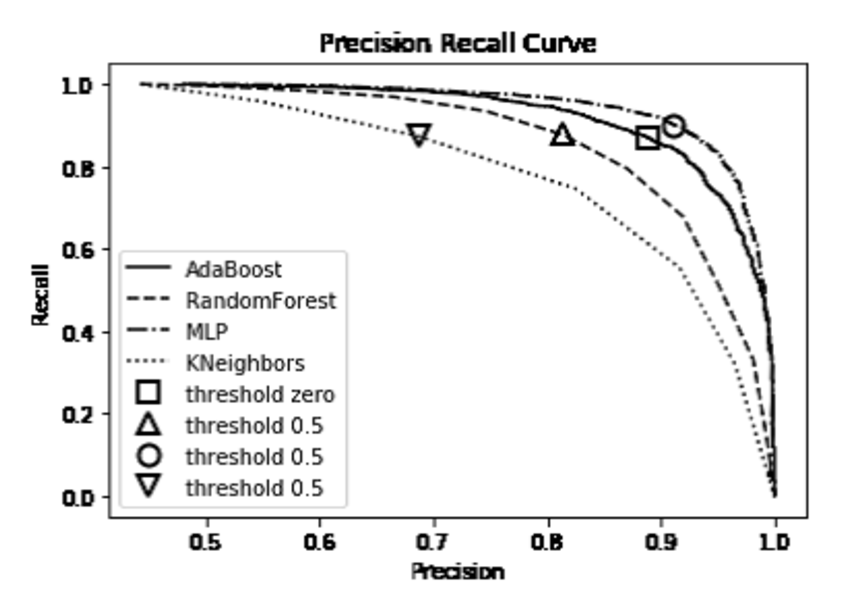
\includegraphics[width=7cm]{./eps/PrecisionRecall_stackoverflow.eps}
    \caption{Precision-recall カーブ}
    \label{tab:nmf_precision}
  \end{center}
\end{figure}
%
\begin{figure}[htb]
  \begin{center}
    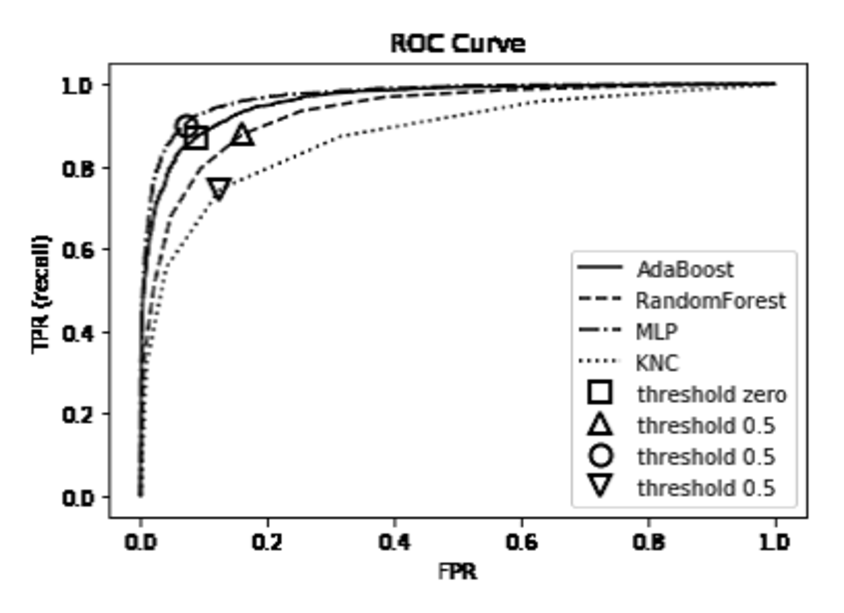
\includegraphics[width=7cm]{./eps/ROC_Curve_stackoverflow.eps}
    \caption{受信者動作特性(ROC)}
    \label{tab:nmf_roc}
  \end{center}
\end{figure}
%
\begin{table}[htb]
  \caption{AUC}
  \label{tab:nmf_auc}
  \begin{center}
  \begin{tabular}{c|c} \hline
    Classification methods & AUC \\ \hline \hline
  AdaBoost & 0.9608 \\ \hline
  RandomForest & 0.9313 \\ \hline
  MLP & 0.9725 \\ \hline
  K-NN & 0.8747 \\ \hline
  \end{tabular}
  \end{center}
\end{table}

結果,分類スレッショルドの最適化を行うことで,
適合率や再現率,F値などの最適化が行える特徴量選択であることが明らかになった.
したがって,提案手法による基底選択は,
文書分類に有効な特徴量を評価する手法としての有効性があると言える.
また,結果から,AUCでは,MLPが最も良いスコアの分類器であることが明らかになった.

%7
\section{まとめ}
本研究では,オンラインコミュニティの質問記事を対象に
既存研究の表層情報,語種や品詞,
文末表現などの2,000次元を越える特徴量に
NMFを適用し,閲覧数を正解データとして基底を評価した.
%
そして,NMFの結果である基底を係数値の差に基づいて評価し,
話題性に影響の大きい基底を評価する方法を提案した.
%\newpage

提案手法で得られた基底に寄与率の高い特徴量を用いて,
話題性の予測と文書分類で評価した.
%
話題性の予測では,SVRで閲覧数に対する予測誤差を算出し,
すべての特徴量を用いた場合比較し,
MAEおよびRMSEの評価指標を評価基準とした.
%
文書分類では,
AdaBoost,RandomForest,MLP,
K-NNの4種類の分類器を用いて,
投稿されたコンテンツのテキスト情報から,
閲覧数が多い話題性のある質問記事と,
閲覧数が少ない質問記事の分類を評価基準とした.
%\newpage
%
評価実験では,ゼネラル・メディアに相当するAppleサポートコミュニティと,
クラス・メディアに相当するStack ExchangeのQ\&Aコミュニティの一つであるstack overflowの
2種類の特性の異なるオンラインコミュニティを用いて提案手法を評価した.

\newpage
非線形回帰を用いた評価では,話題性の予測において,
Appleサポートコミュニティでは,限定的な結果であった.
一方で,stack overflowでは,明瞭な有効性が得られた.
%
分類器を用いた評価では,文書分類において,
Appleサポートコミュニティでは,平均値では分類困難な結果であった.
一方で,stack overflowでは,F値で$0.8$以上の,明瞭な有効性が得られた.
また,すべての特徴量を用いた場合においても有効な結果が得られた.

考察では,オンラインコミュニティの考察を行い,
不満買取センターに投稿される不満投稿に基づいて,
コンテンツが広範なゼネラル・メディアのオンラインコミュニティの場合,
オンラインコミュニティの各カテゴリが,クラス・メディアに相当することが明らかになった.
%
そして,メディアの性質で特徴的な単語が,異なること結果であることが推定できた.
ゆえに,評価実験において,ゼネラル・メディアとクラス・メディアで,
結果に差が出たことは,妥当であることが明らかとなった.
%
加えて,明瞭な結果が得られたstack overflowにおいて,
Precision-recall カーブや,ROCカーブの結果から,
分類器のパラメータや分類スレッショルドを最適化することで,
既存手法よりも良い分類結果を得られることが明らかになった.

今後の課題は,分類基準となる質問記事をラベリングする基準,
分類器のパラメータや分類スレッショルドを最適化である.
さらに,ベイジアンネットワークによる状況変数との
因果関係の推定などでも基底選択の有効性を評価したい.

%8
\section{謝辞}
本研究に連関した研究協力および研究助成頂いた皆様に御礼申し上げます.
本研究における評価結果の考察に際しては,
株式会社Insight Techが国立情報学研究所の協力により,
研究目的で提供している「不満調査データセット」から,
不満カテゴリ辞書データを利用した.
ここに記してデータ提供頂いた株式会社Insight Techに感謝申し上げます.

%\bibliographystyle{jsik}
\bibliographystyle{junsrt}
\bibliography{jsik-bibliography}


%\end{thebibliography}
\end{document}